\documentclass[1p]{elsarticle_modified}
%\bibliographystyle{elsarticle-num}

%\usepackage[colorlinks]{hyperref}
%\usepackage{abbrmath_seonhwa} %\Abb, \Ascr, \Acal ,\Abf, \Afrak
\usepackage{amsfonts}
\usepackage{amssymb}
\usepackage{amsmath}
\usepackage{amsthm}
\usepackage{scalefnt}
\usepackage{amsbsy}
\usepackage{kotex}
\usepackage{caption}
\usepackage{subfig}
\usepackage{color}
\usepackage{graphicx}
\usepackage{xcolor} %% white, black, red, green, blue, cyan, magenta, yellow
\usepackage{float}
\usepackage{setspace}
\usepackage{hyperref}

\usepackage{tikz}
\usetikzlibrary{arrows}

\usepackage{multirow}
\usepackage{array} % fixed length table
\usepackage{hhline}

%%%%%%%%%%%%%%%%%%%%%
\makeatletter
\renewcommand*\env@matrix[1][\arraystretch]{%
	\edef\arraystretch{#1}%
	\hskip -\arraycolsep
	\let\@ifnextchar\new@ifnextchar
	\array{*\c@MaxMatrixCols c}}
\makeatother %https://tex.stackexchange.com/questions/14071/how-can-i-increase-the-line-spacing-in-a-matrix
%%%%%%%%%%%%%%%

\usepackage[normalem]{ulem}

\newcommand{\msout}[1]{\ifmmode\text{\sout{\ensuremath{#1}}}\else\sout{#1}\fi}
%SOURCE: \msout is \stkout macro in https://tex.stackexchange.com/questions/20609/strikeout-in-math-mode

\newcommand{\cancel}[1]{
	\ifmmode
	{\color{red}\msout{#1}}
	\else
	{\color{red}\sout{#1}}
	\fi
}

\newcommand{\add}[1]{
	{\color{blue}\uwave{#1}}
}

\newcommand{\replace}[2]{
	\ifmmode
	{\color{red}\msout{#1}}{\color{blue}\uwave{#2}}
	\else
	{\color{red}\sout{#1}}{\color{blue}\uwave{#2}}
	\fi
}

\newcommand{\Sol}{\mathcal{S}} %segment
\newcommand{\D}{D} %diagram
\newcommand{\A}{\mathcal{A}} %arc


%%%%%%%%%%%%%%%%%%%%%%%%%%%%%5 test

\def\sl{\operatorname{\textup{SL}}(2,\Cbb)}
\def\psl{\operatorname{\textup{PSL}}(2,\Cbb)}
\def\quan{\mkern 1mu \triangleright \mkern 1mu}

\theoremstyle{definition}
\newtheorem{thm}{Theorem}[section]
\newtheorem{prop}[thm]{Proposition}
\newtheorem{lem}[thm]{Lemma}
\newtheorem{ques}[thm]{Question}
\newtheorem{cor}[thm]{Corollary}
\newtheorem{defn}[thm]{Definition}
\newtheorem{exam}[thm]{Example}
\newtheorem{rmk}[thm]{Remark}
\newtheorem{alg}[thm]{Algorithm}

\newcommand{\I}{\sqrt{-1}}
\begin{document}

%\begin{frontmatter}
%
%\title{Boundary parabolic representations of knots up to 8 crossings}
%
%%% Group authors per affiliation:
%\author{Yunhi Cho} 
%\address{Department of Mathematics, University of Seoul, Seoul, Korea}
%\ead{yhcho@uos.ac.kr}
%
%
%\author{Seonhwa Kim} %\fnref{s_kim}}
%\address{Center for Geometry and Physics, Institute for Basic Science, Pohang, 37673, Korea}
%\ead{ryeona17@ibs.re.kr}
%
%\author{Hyuk Kim}
%\address{Department of Mathematical Sciences, Seoul National University, Seoul 08826, Korea}
%\ead{hyukkim@snu.ac.kr}
%
%\author{Seokbeom Yoon}
%\address{Department of Mathematical Sciences, Seoul National University, Seoul, 08826,  Korea}
%\ead{sbyoon15@snu.ac.kr}
%
%\begin{abstract}
%We find all boundary parabolic representation of knots up to 8 crossings.
%
%\end{abstract}
%\begin{keyword}
%    \MSC[2010] 57M25 
%\end{keyword}
%
%\end{frontmatter}

%\linenumbers
%\tableofcontents
%
\newcommand\colored[1]{\textcolor{white}{\rule[-0.35ex]{0.8em}{1.4ex}}\kern-0.8em\color{red} #1}%
%\newcommand\colored[1]{\textcolor{white}{ #1}\kern-2.17ex	\textcolor{white}{ #1}\kern-1.81ex	\textcolor{white}{ #1}\kern-2.15ex\color{red}#1	}

{\Large $\underline{12a_{0618}~(K12a_{0618})}$}

\setlength{\tabcolsep}{10pt}
\renewcommand{\arraystretch}{1.6}
\vspace{1cm}\begin{tabular}{m{100pt}>{\centering\arraybackslash}m{274pt}}
\multirow{5}{120pt}{
	\centering
	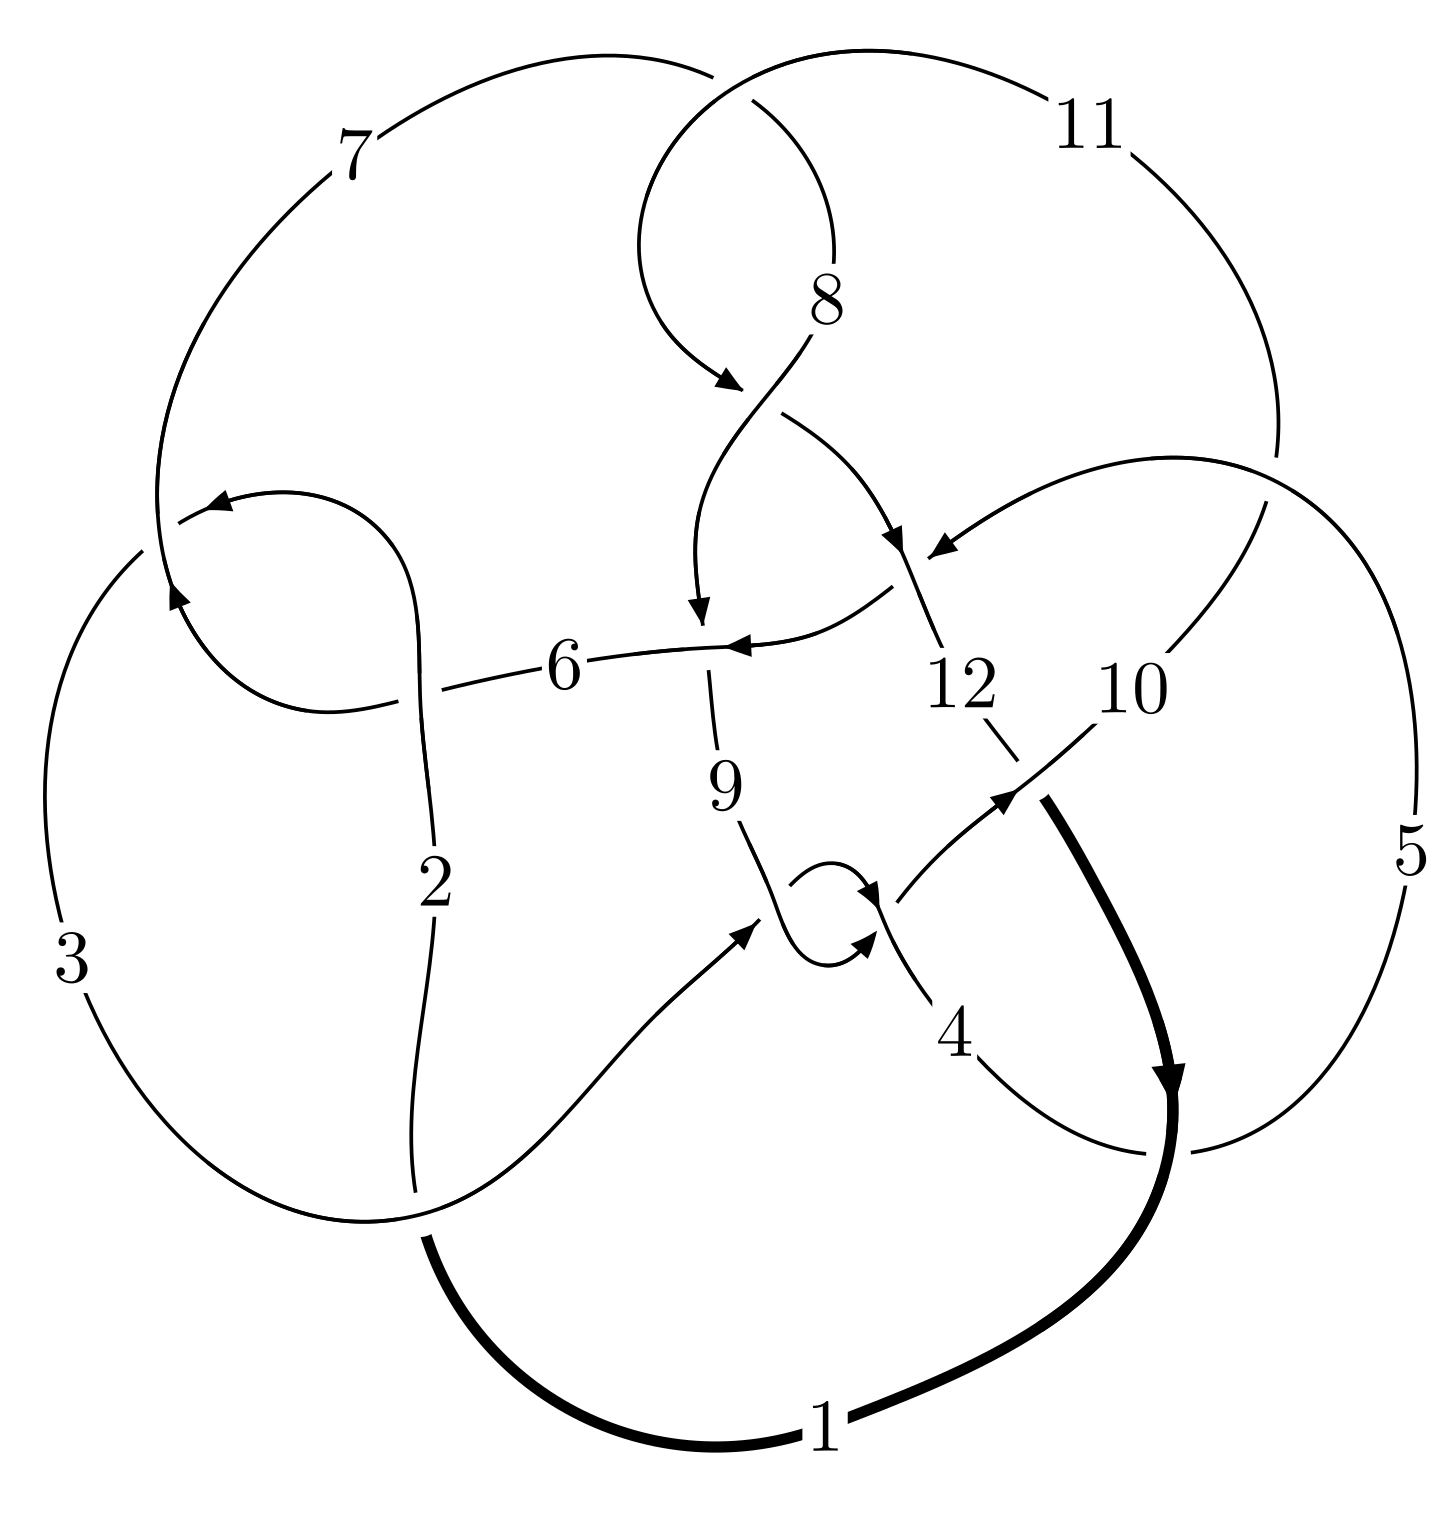
\includegraphics[width=112pt]{../../../GIT/diagram.site/Diagrams/png/1419_12a_0618.png}\\
\ \ \ A knot diagram\footnotemark}&
\allowdisplaybreaks
\textbf{Linearized knot diagam} \\
\cline{2-2}
 &
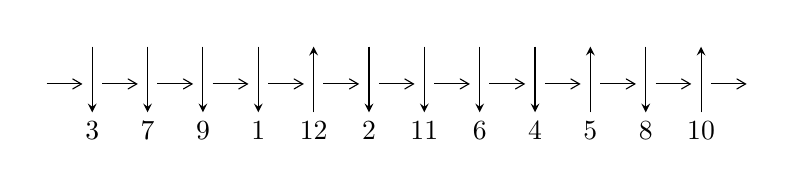
\begin{tikzpicture}[x=20pt, y=17pt]
	% nodes
	\node (C0) at (0, 0) {};
	\node (C1) at (1, 0) {};
	\node (C1U) at (1, +1) {};
	\node (C1D) at (1, -1) {3};

	\node (C2) at (2, 0) {};
	\node (C2U) at (2, +1) {};
	\node (C2D) at (2, -1) {7};

	\node (C3) at (3, 0) {};
	\node (C3U) at (3, +1) {};
	\node (C3D) at (3, -1) {9};

	\node (C4) at (4, 0) {};
	\node (C4U) at (4, +1) {};
	\node (C4D) at (4, -1) {1};

	\node (C5) at (5, 0) {};
	\node (C5U) at (5, +1) {};
	\node (C5D) at (5, -1) {12};

	\node (C6) at (6, 0) {};
	\node (C6U) at (6, +1) {};
	\node (C6D) at (6, -1) {2};

	\node (C7) at (7, 0) {};
	\node (C7U) at (7, +1) {};
	\node (C7D) at (7, -1) {11};

	\node (C8) at (8, 0) {};
	\node (C8U) at (8, +1) {};
	\node (C8D) at (8, -1) {6};

	\node (C9) at (9, 0) {};
	\node (C9U) at (9, +1) {};
	\node (C9D) at (9, -1) {4};

	\node (C10) at (10, 0) {};
	\node (C10U) at (10, +1) {};
	\node (C10D) at (10, -1) {5};

	\node (C11) at (11, 0) {};
	\node (C11U) at (11, +1) {};
	\node (C11D) at (11, -1) {8};

	\node (C12) at (12, 0) {};
	\node (C12U) at (12, +1) {};
	\node (C12D) at (12, -1) {10};
	\node (C13) at (13, 0) {};

	% arrows
	\draw[->,>={angle 60}]
	(C0) edge (C1) (C1) edge (C2) (C2) edge (C3) (C3) edge (C4) (C4) edge (C5) (C5) edge (C6) (C6) edge (C7) (C7) edge (C8) (C8) edge (C9) (C9) edge (C10) (C10) edge (C11) (C11) edge (C12) (C12) edge (C13) ;	\draw[->,>=stealth]
	(C1U) edge (C1D) (C2U) edge (C2D) (C3U) edge (C3D) (C4U) edge (C4D) (C5D) edge (C5U) (C6U) edge (C6D) (C7U) edge (C7D) (C8U) edge (C8D) (C9U) edge (C9D) (C10D) edge (C10U) (C11U) edge (C11D) (C12D) edge (C12U) ;
	\end{tikzpicture} \\
\hhline{~~} \\& 
\textbf{Solving Sequence} \\ \cline{2-2} 
 &
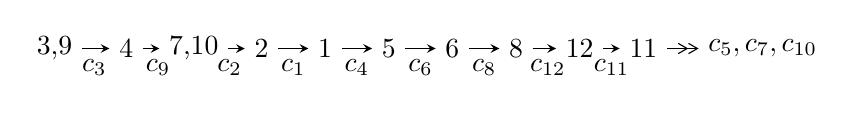
\begin{tikzpicture}[x=23pt, y=7pt]
	% node
	\node (A0) at (-1/8, 0) {3,9};
	\node (A1) at (1, 0) {4};
	\node (A2) at (33/16, 0) {7,10};
	\node (A3) at (25/8, 0) {2};
	\node (A4) at (33/8, 0) {1};
	\node (A5) at (41/8, 0) {5};
	\node (A6) at (49/8, 0) {6};
	\node (A7) at (57/8, 0) {8};
	\node (A8) at (65/8, 0) {12};
	\node (A9) at (73/8, 0) {11};
	\node (C1) at (1/2, -1) {$c_{3}$};
	\node (C2) at (3/2, -1) {$c_{9}$};
	\node (C3) at (21/8, -1) {$c_{2}$};
	\node (C4) at (29/8, -1) {$c_{1}$};
	\node (C5) at (37/8, -1) {$c_{4}$};
	\node (C6) at (45/8, -1) {$c_{6}$};
	\node (C7) at (53/8, -1) {$c_{8}$};
	\node (C8) at (61/8, -1) {$c_{12}$};
	\node (C9) at (69/8, -1) {$c_{11}$};
	\node (A10) at (11, 0) {$c_{5},c_{7},c_{10}$};

	% edge
	\draw[->,>=stealth]	
	(A0) edge (A1) (A1) edge (A2) (A2) edge (A3) (A3) edge (A4) (A4) edge (A5) (A5) edge (A6) (A6) edge (A7) (A7) edge (A8) (A8) edge (A9) ;
	\draw[->>,>={angle 60}]	
	(A9) edge (A10);
\end{tikzpicture} \\ 

\end{tabular} \\

\footnotetext{
The image of knot diagram is generated by the software ``\textbf{Draw programme}" developed by Andrew Bartholomew(\url{http://www.layer8.co.uk/maths/draw/index.htm\#Running-draw}), where we modified some parts for our purpose(\url{https://github.com/CATsTAILs/LinksPainter}).
}\phantom \\ \newline 
\centering \textbf{Ideals for irreducible components\footnotemark of $X_{\text{par}}$} 
 
\begin{align*}
I^u_{1}&=\langle 
2.06637\times10^{1122} u^{171}+5.66934\times10^{1121} u^{170}+\cdots+1.53519\times10^{1123} b-1.66928\times10^{1126},\\
\phantom{I^u_{1}}&\phantom{= \langle  }3.27108\times10^{1126} u^{171}-1.40860\times10^{1126} u^{170}+\cdots+9.43066\times10^{1126} a-9.90581\times10^{1129},\\
\phantom{I^u_{1}}&\phantom{= \langle  }u^{172}- u^{171}+\cdots-565196 u+6143\rangle \\
I^u_{2}&=\langle 
-6.20622\times10^{35} u^{43}+5.45751\times10^{35} u^{42}+\cdots+9.02348\times10^{35} b-3.80488\times10^{36},\\
\phantom{I^u_{2}}&\phantom{= \langle  }-2.88632\times10^{37} u^{43}+2.61790\times10^{37} u^{42}+\cdots+9.92583\times10^{36} a-9.38464\times10^{36},\\
\phantom{I^u_{2}}&\phantom{= \langle  }u^{44}-20 u^{42}+\cdots+6 u+1\rangle \\
\\
\end{align*}
\raggedright * 2 irreducible components of $\dim_{\mathbb{C}}=0$, with total 216 representations.\\
\footnotetext{All coefficients of polynomials are rational numbers. But the coefficients are sometimes approximated in decimal forms when there is not enough margin.}
\newpage
\renewcommand{\arraystretch}{1}
\centering \section*{I. $I^u_{1}= \langle 2.07\times10^{1122} u^{171}+5.67\times10^{1121} u^{170}+\cdots+1.54\times10^{1123} b-1.67\times10^{1126},\;3.27\times10^{1126} u^{171}-1.41\times10^{1126} u^{170}+\cdots+9.43\times10^{1126} a-9.91\times10^{1129},\;u^{172}- u^{171}+\cdots-565196 u+6143 \rangle$}
\flushleft \textbf{(i) Arc colorings}\\
\begin{tabular}{m{7pt} m{180pt} m{7pt} m{180pt} }
\flushright $a_{3}=$&$\begin{pmatrix}1\\0\end{pmatrix}$ \\
\flushright $a_{9}=$&$\begin{pmatrix}0\\u\end{pmatrix}$ \\
\flushright $a_{4}=$&$\begin{pmatrix}1\\u^2\end{pmatrix}$ \\
\flushright $a_{7}=$&$\begin{pmatrix}-0.346856 u^{171}+0.149363 u^{170}+\cdots-98479.0 u+1050.38\\-0.134600 u^{171}-0.0369293 u^{170}+\cdots-99069.3 u+1087.35\end{pmatrix}$ \\
\flushright $a_{10}=$&$\begin{pmatrix}- u\\- u^3+u\end{pmatrix}$ \\
\flushright $a_{2}=$&$\begin{pmatrix}0.157037 u^{171}+0.104546 u^{170}+\cdots+117461. u-1234.56\\0.454629 u^{171}+0.0738660 u^{170}+\cdots+260835. u-2863.48\end{pmatrix}$ \\
\flushright $a_{1}=$&$\begin{pmatrix}0.611666 u^{171}+0.178412 u^{170}+\cdots+378296. u-4098.05\\0.454629 u^{171}+0.0738660 u^{170}+\cdots+260835. u-2863.48\end{pmatrix}$ \\
\flushright $a_{5}=$&$\begin{pmatrix}-0.606909 u^{171}+0.180406 u^{170}+\cdots-201820. u+2162.42\\-0.00630853 u^{171}-0.0496697 u^{170}+\cdots-36441.4 u+399.211\end{pmatrix}$ \\
\flushright $a_{6}=$&$\begin{pmatrix}-0.140540 u^{171}-0.0387226 u^{170}+\cdots-93510.5 u+1042.83\\0.690234 u^{171}+0.128825 u^{170}+\cdots+409669. u-4493.60\end{pmatrix}$ \\
\flushright $a_{8}=$&$\begin{pmatrix}-0.380933 u^{171}-0.190485 u^{170}+\cdots-267616. u+2933.23\\0.0984214 u^{171}+0.0757543 u^{170}+\cdots+97871.5 u-1070.89\end{pmatrix}$ \\
\flushright $a_{12}=$&$\begin{pmatrix}0.230346 u^{171}+0.114479 u^{170}+\cdots+157045. u-1670.25\\0.415235 u^{171}+0.0578417 u^{170}+\cdots+232774. u-2556.09\end{pmatrix}$ \\
\flushright $a_{11}=$&$\begin{pmatrix}0.0205703 u^{171}-0.0861297 u^{170}+\cdots-13104.7 u+183.881\\-0.132302 u^{171}+0.0268440 u^{170}+\cdots-53696.3 u+590.151\end{pmatrix}$\\&\end{tabular}
\flushleft \textbf{(ii) Obstruction class $= -1$}\\~\\
\flushleft \textbf{(iii) Cusp Shapes $= -2.22960 u^{171}-0.108089 u^{170}+\cdots-1.16389\times10^{6} u+12794.1$}\\~\\
\newpage\renewcommand{\arraystretch}{1}
\flushleft \textbf{(iv) u-Polynomials at the component}\newline \\
\begin{tabular}{m{50pt}|m{274pt}}
Crossings & \hspace{64pt}u-Polynomials at each crossing \\
\hline $$\begin{aligned}c_{1}\end{aligned}$$&$\begin{aligned}
&u^{172}+79 u^{171}+\cdots+1449530204 u+56445169
\end{aligned}$\\
\hline $$\begin{aligned}c_{2},c_{6}\end{aligned}$$&$\begin{aligned}
&u^{172}- u^{171}+\cdots-23706 u-7513
\end{aligned}$\\
\hline $$\begin{aligned}c_{3},c_{9}\end{aligned}$$&$\begin{aligned}
&u^{172}- u^{171}+\cdots-565196 u+6143
\end{aligned}$\\
\hline $$\begin{aligned}c_{4}\end{aligned}$$&$\begin{aligned}
&u^{172}-10 u^{171}+\cdots-9148 u+271
\end{aligned}$\\
\hline $$\begin{aligned}c_{5}\end{aligned}$$&$\begin{aligned}
&u^{172}-4 u^{171}+\cdots-11762454 u-858173
\end{aligned}$\\
\hline $$\begin{aligned}c_{7},c_{11}\end{aligned}$$&$\begin{aligned}
&u^{172}+7 u^{171}+\cdots+30336 u+1009
\end{aligned}$\\
\hline $$\begin{aligned}c_{8}\end{aligned}$$&$\begin{aligned}
&u^{172}-5 u^{171}+\cdots-21167440263 u+1101672697
\end{aligned}$\\
\hline $$\begin{aligned}c_{10}\end{aligned}$$&$\begin{aligned}
&u^{172}+u^{171}+\cdots+1522 u-41
\end{aligned}$\\
\hline $$\begin{aligned}c_{12}\end{aligned}$$&$\begin{aligned}
&u^{172}+17 u^{171}+\cdots+493972 u+667
\end{aligned}$\\
\hline
\end{tabular}\\~\\
\newpage\renewcommand{\arraystretch}{1}
\flushleft \textbf{(v) Riley Polynomials at the component}\newline \\
\begin{tabular}{m{50pt}|m{274pt}}
Crossings & \hspace{64pt}Riley Polynomials at each crossing \\
\hline $$\begin{aligned}c_{1}\end{aligned}$$&$\begin{aligned}
&y^{172}+33 y^{171}+\cdots-49226118750771920 y+3186057103438561
\end{aligned}$\\
\hline $$\begin{aligned}c_{2},c_{6}\end{aligned}$$&$\begin{aligned}
&y^{172}-79 y^{171}+\cdots-1449530204 y+56445169
\end{aligned}$\\
\hline $$\begin{aligned}c_{3},c_{9}\end{aligned}$$&$\begin{aligned}
&y^{172}-127 y^{171}+\cdots-334380335706 y+37736449
\end{aligned}$\\
\hline $$\begin{aligned}c_{4}\end{aligned}$$&$\begin{aligned}
&y^{172}-10 y^{171}+\cdots-2951210 y+73441
\end{aligned}$\\
\hline $$\begin{aligned}c_{5}\end{aligned}$$&$\begin{aligned}
&y^{172}+46 y^{171}+\cdots+307627127926670 y+736460897929
\end{aligned}$\\
\hline $$\begin{aligned}c_{7},c_{11}\end{aligned}$$&$\begin{aligned}
&y^{172}-99 y^{171}+\cdots-261670344 y+1018081
\end{aligned}$\\
\hline $$\begin{aligned}c_{8}\end{aligned}$$&$\begin{aligned}
&y^{172}-43 y^{171}+\cdots-9.57\times10^{19} y+1.21\times10^{18}
\end{aligned}$\\
\hline $$\begin{aligned}c_{10}\end{aligned}$$&$\begin{aligned}
&y^{172}-23 y^{171}+\cdots-3429060 y+1681
\end{aligned}$\\
\hline $$\begin{aligned}c_{12}\end{aligned}$$&$\begin{aligned}
&y^{172}+29 y^{171}+\cdots-234106980580 y+444889
\end{aligned}$\\
\hline
\end{tabular}\\~\\
\newpage\flushleft \textbf{(vi) Complex Volumes and Cusp Shapes}
$$\begin{array}{c|c|c}  
\text{Solutions to }I^u_{1}& \I (\text{vol} + \sqrt{-1}CS) & \text{Cusp shape}\\
 \hline 
\begin{aligned}
u &= \phantom{-}0.998590 + 0.083018 I \\
a &= -2.70315 - 1.43498 I \\
b &= -0.838096 + 0.342183 I\end{aligned}
 & -4.01393 - 5.49936 I & \phantom{-0.000000 } 0 \\ \hline\begin{aligned}
u &= \phantom{-}0.998590 - 0.083018 I \\
a &= -2.70315 + 1.43498 I \\
b &= -0.838096 - 0.342183 I\end{aligned}
 & -4.01393 + 5.49936 I & \phantom{-0.000000 } 0 \\ \hline\begin{aligned}
u &= -0.671216 + 0.734904 I \\
a &= -0.352902 - 0.428254 I \\
b &= \phantom{-}1.018330 + 0.591636 I\end{aligned}
 & \phantom{-}1.007700 - 0.949864 I & \phantom{-0.000000 } 0 \\ \hline\begin{aligned}
u &= -0.671216 - 0.734904 I \\
a &= -0.352902 + 0.428254 I \\
b &= \phantom{-}1.018330 - 0.591636 I\end{aligned}
 & \phantom{-}1.007700 + 0.949864 I & \phantom{-0.000000 } 0 \\ \hline\begin{aligned}
u &= \phantom{-}0.840186 + 0.514785 I \\
a &= -0.88529 + 2.30523 I \\
b &= -0.797168 - 0.308580 I\end{aligned}
 & -3.50219 + 0.65545 I & \phantom{-0.000000 } 0 \\ \hline\begin{aligned}
u &= \phantom{-}0.840186 - 0.514785 I \\
a &= -0.88529 - 2.30523 I \\
b &= -0.797168 + 0.308580 I\end{aligned}
 & -3.50219 - 0.65545 I & \phantom{-0.000000 } 0 \\ \hline\begin{aligned}
u &= -1.017000 + 0.033684 I \\
a &= -1.64594 + 1.48163 I \\
b &= -0.984969 - 0.459473 I\end{aligned}
 & -1.87008 + 0.90962 I & \phantom{-0.000000 } 0 \\ \hline\begin{aligned}
u &= -1.017000 - 0.033684 I \\
a &= -1.64594 - 1.48163 I \\
b &= -0.984969 + 0.459473 I\end{aligned}
 & -1.87008 - 0.90962 I & \phantom{-0.000000 } 0 \\ \hline\begin{aligned}
u &= \phantom{-}0.969751 + 0.311784 I \\
a &= \phantom{-}0.252577 + 0.225147 I \\
b &= -0.384266 - 0.700131 I\end{aligned}
 & -0.08093 - 4.78645 I & \phantom{-0.000000 } 0 \\ \hline\begin{aligned}
u &= \phantom{-}0.969751 - 0.311784 I \\
a &= \phantom{-}0.252577 - 0.225147 I \\
b &= -0.384266 + 0.700131 I\end{aligned}
 & -0.08093 + 4.78645 I & \phantom{-0.000000 } 0\\
 \hline 
 \end{array}$$\newpage$$\begin{array}{c|c|c}  
\text{Solutions to }I^u_{1}& \I (\text{vol} + \sqrt{-1}CS) & \text{Cusp shape}\\
 \hline 
\begin{aligned}
u &= -0.902338 + 0.352876 I \\
a &= \phantom{-}0.535598 + 0.489012 I \\
b &= -0.273026 - 1.110210 I\end{aligned}
 & -0.60716 + 5.91889 I & \phantom{-0.000000 } 0 \\ \hline\begin{aligned}
u &= -0.902338 - 0.352876 I \\
a &= \phantom{-}0.535598 - 0.489012 I \\
b &= -0.273026 + 1.110210 I\end{aligned}
 & -0.60716 - 5.91889 I & \phantom{-0.000000 } 0 \\ \hline\begin{aligned}
u &= -0.958081 + 0.051887 I \\
a &= \phantom{-}0.08488 - 1.58109 I \\
b &= -0.941235 + 0.832001 I\end{aligned}
 & \phantom{-}0.105599 + 0.893550 I & \phantom{-0.000000 } 0 \\ \hline\begin{aligned}
u &= -0.958081 - 0.051887 I \\
a &= \phantom{-}0.08488 + 1.58109 I \\
b &= -0.941235 - 0.832001 I\end{aligned}
 & \phantom{-}0.105599 - 0.893550 I & \phantom{-0.000000 } 0 \\ \hline\begin{aligned}
u &= \phantom{-}1.05279\phantom{ +0.000000I} \\
a &= \phantom{-}0.463582\phantom{ +0.000000I} \\
b &= \phantom{-}1.78832\phantom{ +0.000000I}\end{aligned}
 & -7.87076\phantom{ +0.000000I} & \phantom{-0.000000 } 0 \\ \hline\begin{aligned}
u &= -0.907574 + 0.268502 I \\
a &= -0.207023 + 0.209027 I \\
b &= \phantom{-}0.685759 + 0.628492 I\end{aligned}
 & -0.314311 + 0.258798 I & \phantom{-0.000000 } 0 \\ \hline\begin{aligned}
u &= -0.907574 - 0.268502 I \\
a &= -0.207023 - 0.209027 I \\
b &= \phantom{-}0.685759 - 0.628492 I\end{aligned}
 & -0.314311 - 0.258798 I & \phantom{-0.000000 } 0 \\ \hline\begin{aligned}
u &= -1.056610 + 0.006391 I \\
a &= -0.710384 + 0.337117 I \\
b &= \phantom{-}0.479639 - 0.683385 I\end{aligned}
 & -2.04073 - 0.45074 I & \phantom{-0.000000 } 0 \\ \hline\begin{aligned}
u &= -1.056610 - 0.006391 I \\
a &= -0.710384 - 0.337117 I \\
b &= \phantom{-}0.479639 + 0.683385 I\end{aligned}
 & -2.04073 + 0.45074 I & \phantom{-0.000000 } 0 \\ \hline\begin{aligned}
u &= -0.616429 + 0.862114 I \\
a &= \phantom{-}0.773597 + 0.398347 I \\
b &= -0.997849 - 0.055178 I\end{aligned}
 & -5.16587 + 7.46097 I & \phantom{-0.000000 } 0\\
 \hline 
 \end{array}$$\newpage$$\begin{array}{c|c|c}  
\text{Solutions to }I^u_{1}& \I (\text{vol} + \sqrt{-1}CS) & \text{Cusp shape}\\
 \hline 
\begin{aligned}
u &= -0.616429 - 0.862114 I \\
a &= \phantom{-}0.773597 - 0.398347 I \\
b &= -0.997849 + 0.055178 I\end{aligned}
 & -5.16587 - 7.46097 I & \phantom{-0.000000 } 0 \\ \hline\begin{aligned}
u &= -1.057080 + 0.114780 I \\
a &= \phantom{-}1.158650 + 0.468383 I \\
b &= \phantom{-}0.941807 - 0.404110 I\end{aligned}
 & -0.826616 + 0.812580 I & \phantom{-0.000000 } 0 \\ \hline\begin{aligned}
u &= -1.057080 - 0.114780 I \\
a &= \phantom{-}1.158650 - 0.468383 I \\
b &= \phantom{-}0.941807 + 0.404110 I\end{aligned}
 & -0.826616 - 0.812580 I & \phantom{-0.000000 } 0 \\ \hline\begin{aligned}
u &= \phantom{-}0.758962 + 0.537007 I \\
a &= \phantom{-}0.638146 - 0.538369 I \\
b &= -0.360538 + 0.711399 I\end{aligned}
 & \phantom{-}2.49080 - 1.08580 I & \phantom{-0.000000 } 0 \\ \hline\begin{aligned}
u &= \phantom{-}0.758962 - 0.537007 I \\
a &= \phantom{-}0.638146 + 0.538369 I \\
b &= -0.360538 - 0.711399 I\end{aligned}
 & \phantom{-}2.49080 + 1.08580 I & \phantom{-0.000000 } 0 \\ \hline\begin{aligned}
u &= \phantom{-}0.918625 + 0.567748 I \\
a &= -0.359273 - 0.525823 I \\
b &= \phantom{-}0.865900 - 0.398912 I\end{aligned}
 & -0.57933 + 2.45902 I & \phantom{-0.000000 } 0 \\ \hline\begin{aligned}
u &= \phantom{-}0.918625 - 0.567748 I \\
a &= -0.359273 + 0.525823 I \\
b &= \phantom{-}0.865900 + 0.398912 I\end{aligned}
 & -0.57933 - 2.45902 I & \phantom{-0.000000 } 0 \\ \hline\begin{aligned}
u &= \phantom{-}1.080630 + 0.095630 I \\
a &= -0.857223 + 0.793288 I \\
b &= -1.43812 - 0.46639 I\end{aligned}
 & -7.17053 - 0.75192 I & \phantom{-0.000000 } 0 \\ \hline\begin{aligned}
u &= \phantom{-}1.080630 - 0.095630 I \\
a &= -0.857223 - 0.793288 I \\
b &= -1.43812 + 0.46639 I\end{aligned}
 & -7.17053 + 0.75192 I & \phantom{-0.000000 } 0 \\ \hline\begin{aligned}
u &= \phantom{-}0.899924 + 0.111700 I \\
a &= \phantom{-}0.808056 + 0.990079 I \\
b &= -0.815202 - 0.803021 I\end{aligned}
 & \phantom{-}0.45794 - 5.21108 I & \phantom{-0.000000 } 0\\
 \hline 
 \end{array}$$\newpage$$\begin{array}{c|c|c}  
\text{Solutions to }I^u_{1}& \I (\text{vol} + \sqrt{-1}CS) & \text{Cusp shape}\\
 \hline 
\begin{aligned}
u &= \phantom{-}0.899924 - 0.111700 I \\
a &= \phantom{-}0.808056 - 0.990079 I \\
b &= -0.815202 + 0.803021 I\end{aligned}
 & \phantom{-}0.45794 + 5.21108 I & \phantom{-0.000000 } 0 \\ \hline\begin{aligned}
u &= -0.023761 + 1.095910 I \\
a &= -0.13852 + 1.48753 I \\
b &= \phantom{-}0.534497 - 0.796796 I\end{aligned}
 & \phantom{-}0.23858 - 8.55795 I & \phantom{-0.000000 } 0 \\ \hline\begin{aligned}
u &= -0.023761 - 1.095910 I \\
a &= -0.13852 - 1.48753 I \\
b &= \phantom{-}0.534497 + 0.796796 I\end{aligned}
 & \phantom{-}0.23858 + 8.55795 I & \phantom{-0.000000 } 0 \\ \hline\begin{aligned}
u &= -0.350017 + 0.831037 I \\
a &= \phantom{-}1.00244 - 1.73243 I \\
b &= -0.834234 + 0.742856 I\end{aligned}
 & \phantom{-}1.071920 + 0.352220 I & \phantom{-0.000000 } 0 \\ \hline\begin{aligned}
u &= -0.350017 - 0.831037 I \\
a &= \phantom{-}1.00244 + 1.73243 I \\
b &= -0.834234 - 0.742856 I\end{aligned}
 & \phantom{-}1.071920 - 0.352220 I & \phantom{-0.000000 } 0 \\ \hline\begin{aligned}
u &= -1.090900 + 0.139400 I \\
a &= \phantom{-}0.016464 - 0.677979 I \\
b &= -0.55127 + 1.34233 I\end{aligned}
 & -3.24330 + 6.85137 I & \phantom{-0.000000 } 0 \\ \hline\begin{aligned}
u &= -1.090900 - 0.139400 I \\
a &= \phantom{-}0.016464 + 0.677979 I \\
b &= -0.55127 - 1.34233 I\end{aligned}
 & -3.24330 - 6.85137 I & \phantom{-0.000000 } 0 \\ \hline\begin{aligned}
u &= \phantom{-}1.102380 + 0.019608 I \\
a &= -1.170270 + 0.218937 I \\
b &= \phantom{-}0.413295 - 0.730782 I\end{aligned}
 & -4.70366 - 4.85783 I & \phantom{-0.000000 } 0 \\ \hline\begin{aligned}
u &= \phantom{-}1.102380 - 0.019608 I \\
a &= -1.170270 - 0.218937 I \\
b &= \phantom{-}0.413295 + 0.730782 I\end{aligned}
 & -4.70366 + 4.85783 I & \phantom{-0.000000 } 0 \\ \hline\begin{aligned}
u &= -0.972081 + 0.541376 I \\
a &= -0.66541 - 1.60487 I \\
b &= -1.154500 + 0.536515 I\end{aligned}
 & \phantom{-}0.10544 + 5.89897 I & \phantom{-0.000000 } 0\\
 \hline 
 \end{array}$$\newpage$$\begin{array}{c|c|c}  
\text{Solutions to }I^u_{1}& \I (\text{vol} + \sqrt{-1}CS) & \text{Cusp shape}\\
 \hline 
\begin{aligned}
u &= -0.972081 - 0.541376 I \\
a &= -0.66541 + 1.60487 I \\
b &= -1.154500 - 0.536515 I\end{aligned}
 & \phantom{-}0.10544 - 5.89897 I & \phantom{-0.000000 } 0 \\ \hline\begin{aligned}
u &= \phantom{-}0.851388 + 0.721308 I \\
a &= \phantom{-}0.210838 - 1.081940 I \\
b &= \phantom{-}0.575580 + 0.629970 I\end{aligned}
 & \phantom{-}2.34860 - 3.86760 I & \phantom{-0.000000 } 0 \\ \hline\begin{aligned}
u &= \phantom{-}0.851388 - 0.721308 I \\
a &= \phantom{-}0.210838 + 1.081940 I \\
b &= \phantom{-}0.575580 - 0.629970 I\end{aligned}
 & \phantom{-}2.34860 + 3.86760 I & \phantom{-0.000000 } 0 \\ \hline\begin{aligned}
u &= \phantom{-}0.355867 + 0.805051 I \\
a &= -0.767638 + 0.555425 I \\
b &= \phantom{-}1.071560 - 0.641416 I\end{aligned}
 & -1.21606 + 7.47943 I & \phantom{-0.000000 } 0 \\ \hline\begin{aligned}
u &= \phantom{-}0.355867 - 0.805051 I \\
a &= -0.767638 - 0.555425 I \\
b &= \phantom{-}1.071560 + 0.641416 I\end{aligned}
 & -1.21606 - 7.47943 I & \phantom{-0.000000 } 0 \\ \hline\begin{aligned}
u &= -1.122630 + 0.179327 I \\
a &= \phantom{-}0.90061 + 2.22103 I \\
b &= \phantom{-}1.104150 - 0.601771 I\end{aligned}
 & -6.71802 + 9.97895 I & \phantom{-0.000000 } 0 \\ \hline\begin{aligned}
u &= -1.122630 - 0.179327 I \\
a &= \phantom{-}0.90061 - 2.22103 I \\
b &= \phantom{-}1.104150 + 0.601771 I\end{aligned}
 & -6.71802 - 9.97895 I & \phantom{-0.000000 } 0 \\ \hline\begin{aligned}
u &= \phantom{-}1.135510 + 0.072608 I \\
a &= -0.706587 - 1.095310 I \\
b &= \phantom{-}0.474319 + 0.587346 I\end{aligned}
 & -5.57452 - 2.69571 I & \phantom{-0.000000 } 0 \\ \hline\begin{aligned}
u &= \phantom{-}1.135510 - 0.072608 I \\
a &= -0.706587 + 1.095310 I \\
b &= \phantom{-}0.474319 - 0.587346 I\end{aligned}
 & -5.57452 + 2.69571 I & \phantom{-0.000000 } 0 \\ \hline\begin{aligned}
u &= \phantom{-}1.128100 + 0.150398 I \\
a &= \phantom{-}1.15262 - 0.98837 I \\
b &= \phantom{-}0.966602 + 0.612007 I\end{aligned}
 & -1.17125 - 5.16205 I & \phantom{-0.000000 } 0\\
 \hline 
 \end{array}$$\newpage$$\begin{array}{c|c|c}  
\text{Solutions to }I^u_{1}& \I (\text{vol} + \sqrt{-1}CS) & \text{Cusp shape}\\
 \hline 
\begin{aligned}
u &= \phantom{-}1.128100 - 0.150398 I \\
a &= \phantom{-}1.15262 + 0.98837 I \\
b &= \phantom{-}0.966602 - 0.612007 I\end{aligned}
 & -1.17125 + 5.16205 I & \phantom{-0.000000 } 0 \\ \hline\begin{aligned}
u &= -0.042131 + 0.860814 I \\
a &= \phantom{-}0.44215 - 1.48535 I \\
b &= -0.931653 + 0.700856 I\end{aligned}
 & \phantom{-}2.93049 + 3.20631 I & \phantom{-0.000000 } 0 \\ \hline\begin{aligned}
u &= -0.042131 - 0.860814 I \\
a &= \phantom{-}0.44215 + 1.48535 I \\
b &= -0.931653 - 0.700856 I\end{aligned}
 & \phantom{-}2.93049 - 3.20631 I & \phantom{-0.000000 } 0 \\ \hline\begin{aligned}
u &= \phantom{-}0.384843 + 0.770500 I \\
a &= \phantom{-}1.24256 + 1.42581 I \\
b &= -0.932114 - 0.593403 I\end{aligned}
 & \phantom{-}0.75465 - 1.94944 I & \phantom{-0.000000 } 0 \\ \hline\begin{aligned}
u &= \phantom{-}0.384843 - 0.770500 I \\
a &= \phantom{-}1.24256 - 1.42581 I \\
b &= -0.932114 + 0.593403 I\end{aligned}
 & \phantom{-}0.75465 + 1.94944 I & \phantom{-0.000000 } 0 \\ \hline\begin{aligned}
u &= \phantom{-}1.145900 + 0.180926 I \\
a &= \phantom{-}0.73810 - 1.83195 I \\
b &= \phantom{-}1.041890 + 0.599815 I\end{aligned}
 & -3.64420 - 5.41523 I & \phantom{-0.000000 } 0 \\ \hline\begin{aligned}
u &= \phantom{-}1.145900 - 0.180926 I \\
a &= \phantom{-}0.73810 + 1.83195 I \\
b &= \phantom{-}1.041890 - 0.599815 I\end{aligned}
 & -3.64420 + 5.41523 I & \phantom{-0.000000 } 0 \\ \hline\begin{aligned}
u &= -1.149230 + 0.230360 I \\
a &= \phantom{-}0.18034 + 1.95929 I \\
b &= \phantom{-}1.022580 - 0.483336 I\end{aligned}
 & -7.21720 + 1.49192 I & \phantom{-0.000000 } 0 \\ \hline\begin{aligned}
u &= -1.149230 - 0.230360 I \\
a &= \phantom{-}0.18034 - 1.95929 I \\
b &= \phantom{-}1.022580 + 0.483336 I\end{aligned}
 & -7.21720 - 1.49192 I & \phantom{-0.000000 } 0 \\ \hline\begin{aligned}
u &= -0.151449 + 0.803928 I \\
a &= \phantom{-}0.42985 - 1.47905 I \\
b &= -0.753373 + 0.771225 I\end{aligned}
 & \phantom{-}3.47545 + 2.34473 I & \phantom{-0.000000 } 0\\
 \hline 
 \end{array}$$\newpage$$\begin{array}{c|c|c}  
\text{Solutions to }I^u_{1}& \I (\text{vol} + \sqrt{-1}CS) & \text{Cusp shape}\\
 \hline 
\begin{aligned}
u &= -0.151449 - 0.803928 I \\
a &= \phantom{-}0.42985 + 1.47905 I \\
b &= -0.753373 - 0.771225 I\end{aligned}
 & \phantom{-}3.47545 - 2.34473 I & \phantom{-0.000000 } 0 \\ \hline\begin{aligned}
u &= \phantom{-}0.327063 + 0.746465 I \\
a &= \phantom{-}0.64210 - 2.14956 I \\
b &= -0.890841 + 0.744951 I\end{aligned}
 & \phantom{-}0.91188 + 5.28410 I & \phantom{-0.000000 } 0 \\ \hline\begin{aligned}
u &= \phantom{-}0.327063 - 0.746465 I \\
a &= \phantom{-}0.64210 + 2.14956 I \\
b &= -0.890841 - 0.744951 I\end{aligned}
 & \phantom{-}0.91188 - 5.28410 I & \phantom{-0.000000 } 0 \\ \hline\begin{aligned}
u &= -0.542555 + 0.601420 I \\
a &= \phantom{-}0.601527 + 1.247000 I \\
b &= \phantom{-}0.534772 - 0.819837 I\end{aligned}
 & \phantom{-}0.41977 - 2.01791 I & \phantom{-0.000000 } 0 \\ \hline\begin{aligned}
u &= -0.542555 - 0.601420 I \\
a &= \phantom{-}0.601527 - 1.247000 I \\
b &= \phantom{-}0.534772 + 0.819837 I\end{aligned}
 & \phantom{-}0.41977 + 2.01791 I & \phantom{-0.000000 } 0 \\ \hline\begin{aligned}
u &= \phantom{-}0.114065 + 1.190940 I \\
a &= -0.115655 - 1.272080 I \\
b &= \phantom{-}0.614371 + 0.627266 I\end{aligned}
 & \phantom{-}3.11305 + 2.49566 I & \phantom{-0.000000 } 0 \\ \hline\begin{aligned}
u &= \phantom{-}0.114065 - 1.190940 I \\
a &= -0.115655 + 1.272080 I \\
b &= \phantom{-}0.614371 - 0.627266 I\end{aligned}
 & \phantom{-}3.11305 - 2.49566 I & \phantom{-0.000000 } 0 \\ \hline\begin{aligned}
u &= \phantom{-}0.801618\phantom{ +0.000000I} \\
a &= -1.81982\phantom{ +0.000000I} \\
b &= -1.50325\phantom{ +0.000000I}\end{aligned}
 & -7.00476\phantom{ +0.000000I} & \phantom{-0.000000 } 0 \\ \hline\begin{aligned}
u &= \phantom{-}1.148720 + 0.345750 I \\
a &= -0.261247 + 0.324088 I \\
b &= \phantom{-}0.169590 - 0.985522 I\end{aligned}
 & \phantom{-}0.10710 - 5.28156 I & \phantom{-0.000000 } 0 \\ \hline\begin{aligned}
u &= \phantom{-}1.148720 - 0.345750 I \\
a &= -0.261247 - 0.324088 I \\
b &= \phantom{-}0.169590 + 0.985522 I\end{aligned}
 & \phantom{-}0.10710 + 5.28156 I & \phantom{-0.000000 } 0\\
 \hline 
 \end{array}$$\newpage$$\begin{array}{c|c|c}  
\text{Solutions to }I^u_{1}& \I (\text{vol} + \sqrt{-1}CS) & \text{Cusp shape}\\
 \hline 
\begin{aligned}
u &= \phantom{-}1.108760 + 0.472888 I \\
a &= -0.58310 + 1.42647 I \\
b &= -1.239820 - 0.677361 I\end{aligned}
 & -3.52735 - 12.20950 I & \phantom{-0.000000 } 0 \\ \hline\begin{aligned}
u &= \phantom{-}1.108760 - 0.472888 I \\
a &= -0.58310 - 1.42647 I \\
b &= -1.239820 + 0.677361 I\end{aligned}
 & -3.52735 + 12.20950 I & \phantom{-0.000000 } 0 \\ \hline\begin{aligned}
u &= \phantom{-}1.20705\phantom{ +0.000000I} \\
a &= -1.32736\phantom{ +0.000000I} \\
b &= -1.27163\phantom{ +0.000000I}\end{aligned}
 & -6.35449\phantom{ +0.000000I} & \phantom{-0.000000 } 0 \\ \hline\begin{aligned}
u &= \phantom{-}1.103180 + 0.502200 I \\
a &= -0.991477 - 0.358403 I \\
b &= \phantom{-}0.793961 - 0.400031 I\end{aligned}
 & -1.44409 - 2.82165 I & \phantom{-0.000000 } 0 \\ \hline\begin{aligned}
u &= \phantom{-}1.103180 - 0.502200 I \\
a &= -0.991477 + 0.358403 I \\
b &= \phantom{-}0.793961 + 0.400031 I\end{aligned}
 & -1.44409 + 2.82165 I & \phantom{-0.000000 } 0 \\ \hline\begin{aligned}
u &= \phantom{-}0.109090 + 0.772843 I \\
a &= \phantom{-}0.419557 + 1.171380 I \\
b &= -1.037470 - 0.634989 I\end{aligned}
 & \phantom{-}1.59568 - 6.71993 I & \phantom{-0.000000 } 0 \\ \hline\begin{aligned}
u &= \phantom{-}0.109090 - 0.772843 I \\
a &= \phantom{-}0.419557 - 1.171380 I \\
b &= -1.037470 + 0.634989 I\end{aligned}
 & \phantom{-}1.59568 + 6.71993 I & \phantom{-0.000000 } 0 \\ \hline\begin{aligned}
u &= -1.22022\phantom{ +0.000000I} \\
a &= -0.671099\phantom{ +0.000000I} \\
b &= -1.60020\phantom{ +0.000000I}\end{aligned}
 & -6.41930\phantom{ +0.000000I} & \phantom{-0.000000 } 0 \\ \hline\begin{aligned}
u &= -0.042478 + 0.753549 I \\
a &= \phantom{-}0.70835 + 1.40352 I \\
b &= -0.034371 - 0.482778 I\end{aligned}
 & -2.58094 + 0.53449 I & \phantom{-0.000000 } 0 \\ \hline\begin{aligned}
u &= -0.042478 - 0.753549 I \\
a &= \phantom{-}0.70835 - 1.40352 I \\
b &= -0.034371 + 0.482778 I\end{aligned}
 & -2.58094 - 0.53449 I & \phantom{-0.000000 } 0\\
 \hline 
 \end{array}$$\newpage$$\begin{array}{c|c|c}  
\text{Solutions to }I^u_{1}& \I (\text{vol} + \sqrt{-1}CS) & \text{Cusp shape}\\
 \hline 
\begin{aligned}
u &= -0.512305 + 1.144340 I \\
a &= \phantom{-}0.786948 + 1.054200 I \\
b &= -1.011110 - 0.473275 I\end{aligned}
 & -4.67500 - 3.97099 I & \phantom{-0.000000 } 0 \\ \hline\begin{aligned}
u &= -0.512305 - 1.144340 I \\
a &= \phantom{-}0.786948 - 1.054200 I \\
b &= -1.011110 + 0.473275 I\end{aligned}
 & -4.67500 + 3.97099 I & \phantom{-0.000000 } 0 \\ \hline\begin{aligned}
u &= -1.148210 + 0.531016 I \\
a &= -1.041120 - 0.136801 I \\
b &= \phantom{-}0.755046 + 0.678130 I\end{aligned}
 & -1.41753 + 4.72367 I & \phantom{-0.000000 } 0 \\ \hline\begin{aligned}
u &= -1.148210 - 0.531016 I \\
a &= -1.041120 + 0.136801 I \\
b &= \phantom{-}0.755046 - 0.678130 I\end{aligned}
 & -1.41753 - 4.72367 I & \phantom{-0.000000 } 0 \\ \hline\begin{aligned}
u &= -1.202760 + 0.410604 I \\
a &= -0.448550 - 0.278364 I \\
b &= \phantom{-}0.522545 + 0.870296 I\end{aligned}
 & \phantom{-}0.21839 + 2.08193 I & \phantom{-0.000000 } 0 \\ \hline\begin{aligned}
u &= -1.202760 - 0.410604 I \\
a &= -0.448550 + 0.278364 I \\
b &= \phantom{-}0.522545 - 0.870296 I\end{aligned}
 & \phantom{-}0.21839 - 2.08193 I & \phantom{-0.000000 } 0 \\ \hline\begin{aligned}
u &= \phantom{-}1.261080 + 0.163710 I \\
a &= \phantom{-}0.217143 - 1.081370 I \\
b &= \phantom{-}0.937483 + 0.914940 I\end{aligned}
 & -4.24744 - 3.11310 I & \phantom{-0.000000 } 0 \\ \hline\begin{aligned}
u &= \phantom{-}1.261080 - 0.163710 I \\
a &= \phantom{-}0.217143 + 1.081370 I \\
b &= \phantom{-}0.937483 - 0.914940 I\end{aligned}
 & -4.24744 + 3.11310 I & \phantom{-0.000000 } 0 \\ \hline\begin{aligned}
u &= -1.269440 + 0.079003 I \\
a &= \phantom{-}0.230927 + 0.872934 I \\
b &= \phantom{-}1.19548 - 0.86969 I\end{aligned}
 & -4.93877 + 4.11641 I & \phantom{-0.000000 } 0 \\ \hline\begin{aligned}
u &= -1.269440 - 0.079003 I \\
a &= \phantom{-}0.230927 - 0.872934 I \\
b &= \phantom{-}1.19548 + 0.86969 I\end{aligned}
 & -4.93877 - 4.11641 I & \phantom{-0.000000 } 0\\
 \hline 
 \end{array}$$\newpage$$\begin{array}{c|c|c}  
\text{Solutions to }I^u_{1}& \I (\text{vol} + \sqrt{-1}CS) & \text{Cusp shape}\\
 \hline 
\begin{aligned}
u &= \phantom{-}1.167760 + 0.549132 I \\
a &= -0.146242 + 1.286230 I \\
b &= \phantom{-}0.382585 - 0.390444 I\end{aligned}
 & -4.53113 + 3.56547 I & \phantom{-0.000000 } 0 \\ \hline\begin{aligned}
u &= \phantom{-}1.167760 - 0.549132 I \\
a &= -0.146242 - 1.286230 I \\
b &= \phantom{-}0.382585 + 0.390444 I\end{aligned}
 & -4.53113 - 3.56547 I & \phantom{-0.000000 } 0 \\ \hline\begin{aligned}
u &= -1.249990 + 0.349953 I \\
a &= \phantom{-}1.62100 + 1.21358 I \\
b &= \phantom{-}0.949362 - 0.457267 I\end{aligned}
 & -2.04894 + 6.40652 I & \phantom{-0.000000 } 0 \\ \hline\begin{aligned}
u &= -1.249990 - 0.349953 I \\
a &= \phantom{-}1.62100 - 1.21358 I \\
b &= \phantom{-}0.949362 + 0.457267 I\end{aligned}
 & -2.04894 - 6.40652 I & \phantom{-0.000000 } 0 \\ \hline\begin{aligned}
u &= -0.085322 + 1.299100 I \\
a &= -0.485765 + 1.230370 I \\
b &= \phantom{-}1.069820 - 0.642227 I\end{aligned}
 & -1.38147 + 13.97860 I & \phantom{-0.000000 } 0 \\ \hline\begin{aligned}
u &= -0.085322 - 1.299100 I \\
a &= -0.485765 - 1.230370 I \\
b &= \phantom{-}1.069820 + 0.642227 I\end{aligned}
 & -1.38147 - 13.97860 I & \phantom{-0.000000 } 0 \\ \hline\begin{aligned}
u &= \phantom{-}1.226950 + 0.435585 I \\
a &= \phantom{-}1.26021 - 1.82680 I \\
b &= \phantom{-}0.941981 + 0.627852 I\end{aligned}
 & -2.00424 - 9.78934 I & \phantom{-0.000000 } 0 \\ \hline\begin{aligned}
u &= \phantom{-}1.226950 - 0.435585 I \\
a &= \phantom{-}1.26021 + 1.82680 I \\
b &= \phantom{-}0.941981 - 0.627852 I\end{aligned}
 & -2.00424 + 9.78934 I & \phantom{-0.000000 } 0 \\ \hline\begin{aligned}
u &= \phantom{-}0.159664 + 0.671926 I \\
a &= \phantom{-}0.143454 + 1.182010 I \\
b &= -0.535188 - 0.757867 I\end{aligned}
 & \phantom{-}3.07778 + 1.44225 I & \phantom{-0.000000 } 0 \\ \hline\begin{aligned}
u &= \phantom{-}0.159664 - 0.671926 I \\
a &= \phantom{-}0.143454 - 1.182010 I \\
b &= -0.535188 + 0.757867 I\end{aligned}
 & \phantom{-}3.07778 - 1.44225 I & \phantom{-0.000000 } 0\\
 \hline 
 \end{array}$$\newpage$$\begin{array}{c|c|c}  
\text{Solutions to }I^u_{1}& \I (\text{vol} + \sqrt{-1}CS) & \text{Cusp shape}\\
 \hline 
\begin{aligned}
u &= \phantom{-}0.259853 + 1.288290 I \\
a &= -0.309473 + 0.724937 I \\
b &= \phantom{-}1.011020 - 0.341449 I\end{aligned}
 & -5.41386 + 2.32416 I & \phantom{-0.000000 } 0 \\ \hline\begin{aligned}
u &= \phantom{-}0.259853 - 1.288290 I \\
a &= -0.309473 - 0.724937 I \\
b &= \phantom{-}1.011020 + 0.341449 I\end{aligned}
 & -5.41386 - 2.32416 I & \phantom{-0.000000 } 0 \\ \hline\begin{aligned}
u &= -1.336930 + 0.057521 I \\
a &= -1.020810 - 0.585017 I \\
b &= -1.165680 - 0.238914 I\end{aligned}
 & -9.28643 + 2.28089 I & \phantom{-0.000000 } 0 \\ \hline\begin{aligned}
u &= -1.336930 - 0.057521 I \\
a &= -1.020810 + 0.585017 I \\
b &= -1.165680 + 0.238914 I\end{aligned}
 & -9.28643 - 2.28089 I & \phantom{-0.000000 } 0 \\ \hline\begin{aligned}
u &= -1.093550 + 0.776338 I \\
a &= -0.47922 - 1.56155 I \\
b &= -0.980501 + 0.417713 I\end{aligned}
 & -0.50308 + 5.35081 I & \phantom{-0.000000 } 0 \\ \hline\begin{aligned}
u &= -1.093550 - 0.776338 I \\
a &= -0.47922 + 1.56155 I \\
b &= -0.980501 - 0.417713 I\end{aligned}
 & -0.50308 - 5.35081 I & \phantom{-0.000000 } 0 \\ \hline\begin{aligned}
u &= -1.254000 + 0.498619 I \\
a &= \phantom{-}0.353611 + 0.779468 I \\
b &= -0.114679 - 0.874953 I\end{aligned}
 & -6.10140 + 4.22576 I & \phantom{-0.000000 } 0 \\ \hline\begin{aligned}
u &= -1.254000 - 0.498619 I \\
a &= \phantom{-}0.353611 - 0.779468 I \\
b &= -0.114679 + 0.874953 I\end{aligned}
 & -6.10140 - 4.22576 I & \phantom{-0.000000 } 0 \\ \hline\begin{aligned}
u &= \phantom{-}1.328680 + 0.297617 I \\
a &= \phantom{-}0.326746 + 0.245963 I \\
b &= \phantom{-}1.308420 - 0.312619 I\end{aligned}
 & -10.72340 + 0.03355 I & \phantom{-0.000000 } 0 \\ \hline\begin{aligned}
u &= \phantom{-}1.328680 - 0.297617 I \\
a &= \phantom{-}0.326746 - 0.245963 I \\
b &= \phantom{-}1.308420 + 0.312619 I\end{aligned}
 & -10.72340 - 0.03355 I & \phantom{-0.000000 } 0\\
 \hline 
 \end{array}$$\newpage$$\begin{array}{c|c|c}  
\text{Solutions to }I^u_{1}& \I (\text{vol} + \sqrt{-1}CS) & \text{Cusp shape}\\
 \hline 
\begin{aligned}
u &= \phantom{-}1.259210 + 0.549836 I \\
a &= -0.724990 + 0.861993 I \\
b &= \phantom{-}0.480409 - 0.824482 I\end{aligned}
 & -5.80576 - 5.37340 I & \phantom{-0.000000 } 0 \\ \hline\begin{aligned}
u &= \phantom{-}1.259210 - 0.549836 I \\
a &= -0.724990 - 0.861993 I \\
b &= \phantom{-}0.480409 + 0.824482 I\end{aligned}
 & -5.80576 + 5.37340 I & \phantom{-0.000000 } 0 \\ \hline\begin{aligned}
u &= \phantom{-}0.799397 + 1.118970 I \\
a &= \phantom{-}0.566525 - 0.757762 I \\
b &= -0.858471 + 0.346278 I\end{aligned}
 & \phantom{-}0.08172 - 2.26660 I & \phantom{-0.000000 } 0 \\ \hline\begin{aligned}
u &= \phantom{-}0.799397 - 1.118970 I \\
a &= \phantom{-}0.566525 + 0.757762 I \\
b &= -0.858471 - 0.346278 I\end{aligned}
 & \phantom{-}0.08172 + 2.26660 I & \phantom{-0.000000 } 0 \\ \hline\begin{aligned}
u &= \phantom{-}1.384640 + 0.082717 I \\
a &= -1.004530 - 0.181068 I \\
b &= -1.068940 - 0.069049 I\end{aligned}
 & -6.89103 - 1.05292 I & \phantom{-0.000000 } 0 \\ \hline\begin{aligned}
u &= \phantom{-}1.384640 - 0.082717 I \\
a &= -1.004530 + 0.181068 I \\
b &= -1.068940 + 0.069049 I\end{aligned}
 & -6.89103 + 1.05292 I & \phantom{-0.000000 } 0 \\ \hline\begin{aligned}
u &= -0.612876\phantom{ +0.000000I} \\
a &= \phantom{-}0.663834\phantom{ +0.000000I} \\
b &= \phantom{-}0.504299\phantom{ +0.000000I}\end{aligned}
 & -0.951403\phantom{ +0.000000I} & \phantom{-0.000000 } 0 \\ \hline\begin{aligned}
u &= -1.336290 + 0.380072 I \\
a &= \phantom{-}0.82342 + 1.18995 I \\
b &= \phantom{-}1.211440 - 0.617972 I\end{aligned}
 & -2.89733 + 10.96930 I & \phantom{-0.000000 } 0 \\ \hline\begin{aligned}
u &= -1.336290 - 0.380072 I \\
a &= \phantom{-}0.82342 - 1.18995 I \\
b &= \phantom{-}1.211440 + 0.617972 I\end{aligned}
 & -2.89733 - 10.96930 I & \phantom{-0.000000 } 0 \\ \hline\begin{aligned}
u &= -1.359100 + 0.289253 I \\
a &= \phantom{-}0.625095 - 0.099927 I \\
b &= \phantom{-}1.242870 + 0.092408 I\end{aligned}
 & -6.61459 + 5.82404 I & \phantom{-0.000000 } 0\\
 \hline 
 \end{array}$$\newpage$$\begin{array}{c|c|c}  
\text{Solutions to }I^u_{1}& \I (\text{vol} + \sqrt{-1}CS) & \text{Cusp shape}\\
 \hline 
\begin{aligned}
u &= -1.359100 - 0.289253 I \\
a &= \phantom{-}0.625095 + 0.099927 I \\
b &= \phantom{-}1.242870 - 0.092408 I\end{aligned}
 & -6.61459 - 5.82404 I & \phantom{-0.000000 } 0 \\ \hline\begin{aligned}
u &= \phantom{-}1.364230 + 0.294735 I \\
a &= \phantom{-}0.500379 - 0.199704 I \\
b &= \phantom{-}1.401460 + 0.021802 I\end{aligned}
 & -11.1084 - 10.9874 I & \phantom{-0.000000 } 0 \\ \hline\begin{aligned}
u &= \phantom{-}1.364230 - 0.294735 I \\
a &= \phantom{-}0.500379 + 0.199704 I \\
b &= \phantom{-}1.401460 - 0.021802 I\end{aligned}
 & -11.1084 + 10.9874 I & \phantom{-0.000000 } 0 \\ \hline\begin{aligned}
u &= \phantom{-}1.349580 + 0.406070 I \\
a &= \phantom{-}0.82516 - 1.34911 I \\
b &= \phantom{-}1.085380 + 0.678313 I\end{aligned}
 & -1.47869 - 7.80448 I & \phantom{-0.000000 } 0 \\ \hline\begin{aligned}
u &= \phantom{-}1.349580 - 0.406070 I \\
a &= \phantom{-}0.82516 + 1.34911 I \\
b &= \phantom{-}1.085380 - 0.678313 I\end{aligned}
 & -1.47869 + 7.80448 I & \phantom{-0.000000 } 0 \\ \hline\begin{aligned}
u &= -1.31980 + 0.52740 I \\
a &= -0.337232 - 0.729937 I \\
b &= \phantom{-}0.579825 + 0.683070 I\end{aligned}
 & -1.52491 + 1.56540 I & \phantom{-0.000000 } 0 \\ \hline\begin{aligned}
u &= -1.31980 - 0.52740 I \\
a &= -0.337232 + 0.729937 I \\
b &= \phantom{-}0.579825 - 0.683070 I\end{aligned}
 & -1.52491 - 1.56540 I & \phantom{-0.000000 } 0 \\ \hline\begin{aligned}
u &= -0.243701 + 0.523659 I \\
a &= -0.19023 + 2.63527 I \\
b &= -0.786842 - 0.641066 I\end{aligned}
 & \phantom{-}1.23767 - 2.89064 I & \phantom{-0.000000 } 0 \\ \hline\begin{aligned}
u &= -0.243701 - 0.523659 I \\
a &= -0.19023 - 2.63527 I \\
b &= -0.786842 + 0.641066 I\end{aligned}
 & \phantom{-}1.23767 + 2.89064 I & \phantom{-0.000000 } 0 \\ \hline\begin{aligned}
u &= \phantom{-}0.351885 + 0.448093 I \\
a &= -0.114027 - 0.308074 I \\
b &= \phantom{-}0.062567 - 0.530066 I\end{aligned}
 & \phantom{-}1.44477 + 1.59152 I & \phantom{-0.000000 } 0\\
 \hline 
 \end{array}$$\newpage$$\begin{array}{c|c|c}  
\text{Solutions to }I^u_{1}& \I (\text{vol} + \sqrt{-1}CS) & \text{Cusp shape}\\
 \hline 
\begin{aligned}
u &= \phantom{-}0.351885 - 0.448093 I \\
a &= -0.114027 + 0.308074 I \\
b &= \phantom{-}0.062567 + 0.530066 I\end{aligned}
 & \phantom{-}1.44477 - 1.59152 I & \phantom{-0.000000 } 0 \\ \hline\begin{aligned}
u &= -0.505387 + 0.259815 I \\
a &= \phantom{-}0.562521 - 0.450150 I \\
b &= \phantom{-}0.737299 - 0.072449 I\end{aligned}
 & -1.149250 + 0.056990 I & \phantom{-0.000000 } 0 \\ \hline\begin{aligned}
u &= -0.505387 - 0.259815 I \\
a &= \phantom{-}0.562521 + 0.450150 I \\
b &= \phantom{-}0.737299 + 0.072449 I\end{aligned}
 & -1.149250 - 0.056990 I & \phantom{-0.000000 } 0 \\ \hline\begin{aligned}
u &= \phantom{-}0.10760 + 1.43221 I \\
a &= -0.339211 - 1.136350 I \\
b &= \phantom{-}0.992436 + 0.581582 I\end{aligned}
 & \phantom{-}1.97716 - 7.26559 I & \phantom{-0.000000 } 0 \\ \hline\begin{aligned}
u &= \phantom{-}0.10760 - 1.43221 I \\
a &= -0.339211 + 1.136350 I \\
b &= \phantom{-}0.992436 - 0.581582 I\end{aligned}
 & \phantom{-}1.97716 + 7.26559 I & \phantom{-0.000000 } 0 \\ \hline\begin{aligned}
u &= \phantom{-}1.32344 + 0.55896 I \\
a &= \phantom{-}0.443021 - 0.645431 I \\
b &= -0.431089 + 0.880936 I\end{aligned}
 & -0.73057 - 8.49882 I & \phantom{-0.000000 } 0 \\ \hline\begin{aligned}
u &= \phantom{-}1.32344 - 0.55896 I \\
a &= \phantom{-}0.443021 + 0.645431 I \\
b &= -0.431089 - 0.880936 I\end{aligned}
 & -0.73057 + 8.49882 I & \phantom{-0.000000 } 0 \\ \hline\begin{aligned}
u &= -1.34383 + 0.53049 I \\
a &= \phantom{-}0.528385 + 0.663994 I \\
b &= -0.462330 - 1.018120 I\end{aligned}
 & -3.9068 + 14.2702 I & \phantom{-0.000000 } 0 \\ \hline\begin{aligned}
u &= -1.34383 - 0.53049 I \\
a &= \phantom{-}0.528385 - 0.663994 I \\
b &= -0.462330 + 1.018120 I\end{aligned}
 & -3.9068 - 14.2702 I & \phantom{-0.000000 } 0 \\ \hline\begin{aligned}
u &= -0.539194 + 0.114319 I \\
a &= \phantom{-}2.43005 - 1.22633 I \\
b &= -1.024180 - 0.404154 I\end{aligned}
 & -4.76460 - 8.42888 I & \phantom{-0.000000 } 0\\
 \hline 
 \end{array}$$\newpage$$\begin{array}{c|c|c}  
\text{Solutions to }I^u_{1}& \I (\text{vol} + \sqrt{-1}CS) & \text{Cusp shape}\\
 \hline 
\begin{aligned}
u &= -0.539194 - 0.114319 I \\
a &= \phantom{-}2.43005 + 1.22633 I \\
b &= -1.024180 + 0.404154 I\end{aligned}
 & -4.76460 + 8.42888 I & \phantom{-0.000000 } 0 \\ \hline\begin{aligned}
u &= -0.347449 + 0.413474 I \\
a &= \phantom{-}2.91043 - 0.50359 I \\
b &= -0.973884 - 0.146380 I\end{aligned}
 & -4.72180 + 1.18594 I & \phantom{-0.000000 } 0 \\ \hline\begin{aligned}
u &= -0.347449 - 0.413474 I \\
a &= \phantom{-}2.91043 + 0.50359 I \\
b &= -0.973884 + 0.146380 I\end{aligned}
 & -4.72180 - 1.18594 I & \phantom{-0.000000 } 0 \\ \hline\begin{aligned}
u &= -1.50172 + 0.13595 I \\
a &= -0.561304 - 0.159721 I \\
b &= -0.960942 - 0.444610 I\end{aligned}
 & -7.64378 - 4.26202 I & \phantom{-0.000000 } 0 \\ \hline\begin{aligned}
u &= -1.50172 - 0.13595 I \\
a &= -0.561304 + 0.159721 I \\
b &= -0.960942 + 0.444610 I\end{aligned}
 & -7.64378 + 4.26202 I & \phantom{-0.000000 } 0 \\ \hline\begin{aligned}
u &= -1.34715 + 0.68196 I \\
a &= \phantom{-}0.22814 + 1.70279 I \\
b &= \phantom{-}1.101010 - 0.647754 I\end{aligned}
 & -7.66123 + 10.88750 I & \phantom{-0.000000 } 0 \\ \hline\begin{aligned}
u &= -1.34715 - 0.68196 I \\
a &= \phantom{-}0.22814 - 1.70279 I \\
b &= \phantom{-}1.101010 + 0.647754 I\end{aligned}
 & -7.66123 - 10.88750 I & \phantom{-0.000000 } 0 \\ \hline\begin{aligned}
u &= \phantom{-}1.51034 + 0.02862 I \\
a &= -0.956226 + 0.015529 I \\
b &= -0.790805 + 0.378359 I\end{aligned}
 & -6.96844 - 0.80038 I & \phantom{-0.000000 } 0 \\ \hline\begin{aligned}
u &= \phantom{-}1.51034 - 0.02862 I \\
a &= -0.956226 - 0.015529 I \\
b &= -0.790805 - 0.378359 I\end{aligned}
 & -6.96844 + 0.80038 I & \phantom{-0.000000 } 0 \\ \hline\begin{aligned}
u &= \phantom{-}1.38592 + 0.62946 I \\
a &= -0.419266 + 1.334070 I \\
b &= -1.175050 - 0.512438 I\end{aligned}
 & -9.27131 - 9.10281 I & \phantom{-0.000000 } 0\\
 \hline 
 \end{array}$$\newpage$$\begin{array}{c|c|c}  
\text{Solutions to }I^u_{1}& \I (\text{vol} + \sqrt{-1}CS) & \text{Cusp shape}\\
 \hline 
\begin{aligned}
u &= \phantom{-}1.38592 - 0.62946 I \\
a &= -0.419266 - 1.334070 I \\
b &= -1.175050 + 0.512438 I\end{aligned}
 & -9.27131 + 9.10281 I & \phantom{-0.000000 } 0 \\ \hline\begin{aligned}
u &= -1.48744 + 0.34894 I \\
a &= -0.429082 - 0.173192 I \\
b &= -1.187870 - 0.075409 I\end{aligned}
 & -11.48550 + 3.23271 I & \phantom{-0.000000 } 0 \\ \hline\begin{aligned}
u &= -1.48744 - 0.34894 I \\
a &= -0.429082 + 0.173192 I \\
b &= -1.187870 + 0.075409 I\end{aligned}
 & -11.48550 - 3.23271 I & \phantom{-0.000000 } 0 \\ \hline\begin{aligned}
u &= \phantom{-}1.43525 + 0.58085 I \\
a &= -0.47231 + 1.47471 I \\
b &= -1.175510 - 0.697807 I\end{aligned}
 & -6.1324 - 20.4683 I & \phantom{-0.000000 } 0 \\ \hline\begin{aligned}
u &= \phantom{-}1.43525 - 0.58085 I \\
a &= -0.47231 - 1.47471 I \\
b &= -1.175510 + 0.697807 I\end{aligned}
 & -6.1324 + 20.4683 I & \phantom{-0.000000 } 0 \\ \hline\begin{aligned}
u &= -1.44968 + 0.60453 I \\
a &= -0.47889 - 1.40475 I \\
b &= -1.134340 + 0.643643 I\end{aligned}
 & -2.8585 + 14.1270 I & \phantom{-0.000000 } 0 \\ \hline\begin{aligned}
u &= -1.44968 - 0.60453 I \\
a &= -0.47889 + 1.40475 I \\
b &= -1.134340 - 0.643643 I\end{aligned}
 & -2.8585 - 14.1270 I & \phantom{-0.000000 } 0 \\ \hline\begin{aligned}
u &= \phantom{-}0.143722 + 0.343781 I \\
a &= -1.23341 - 0.76427 I \\
b &= \phantom{-}1.163920 - 0.361344 I\end{aligned}
 & -4.68589 - 0.94693 I & -9.76471 + 5.85345 I \\ \hline\begin{aligned}
u &= \phantom{-}0.143722 - 0.343781 I \\
a &= -1.23341 + 0.76427 I \\
b &= \phantom{-}1.163920 + 0.361344 I\end{aligned}
 & -4.68589 + 0.94693 I & -9.76471 - 5.85345 I \\ \hline\begin{aligned}
u &= -0.266154 + 0.172836 I \\
a &= -0.22800 + 1.68476 I \\
b &= \phantom{-}0.189222 + 0.866563 I\end{aligned}
 & -1.14221 - 5.34706 I & -3.94019 + 5.65009 I\\
 \hline 
 \end{array}$$\newpage$$\begin{array}{c|c|c}  
\text{Solutions to }I^u_{1}& \I (\text{vol} + \sqrt{-1}CS) & \text{Cusp shape}\\
 \hline 
\begin{aligned}
u &= -0.266154 - 0.172836 I \\
a &= -0.22800 - 1.68476 I \\
b &= \phantom{-}0.189222 - 0.866563 I\end{aligned}
 & -1.14221 + 5.34706 I & -3.94019 - 5.65009 I \\ \hline\begin{aligned}
u &= \phantom{-}0.287851 + 0.076632 I \\
a &= \phantom{-}2.95502 + 2.92029 I \\
b &= -0.899062 + 0.332036 I\end{aligned}
 & -0.98061 + 3.88705 I & -10.08732 - 6.71034 I \\ \hline\begin{aligned}
u &= \phantom{-}0.287851 - 0.076632 I \\
a &= \phantom{-}2.95502 - 2.92029 I \\
b &= -0.899062 - 0.332036 I\end{aligned}
 & -0.98061 - 3.88705 I & -10.08732 + 6.71034 I \\ \hline\begin{aligned}
u &= \phantom{-}1.60615 + 0.60306 I \\
a &= \phantom{-}0.312232 - 1.298830 I \\
b &= \phantom{-}1.001710 + 0.613928 I\end{aligned}
 & -2.75443 - 6.59029 I & \phantom{-0.000000 } 0 \\ \hline\begin{aligned}
u &= \phantom{-}1.60615 - 0.60306 I \\
a &= \phantom{-}0.312232 + 1.298830 I \\
b &= \phantom{-}1.001710 - 0.613928 I\end{aligned}
 & -2.75443 + 6.59029 I & \phantom{-0.000000 } 0 \\ \hline\begin{aligned}
u &= -1.39519 + 1.19829 I \\
a &= -0.072995 + 1.214310 I \\
b &= \phantom{-}0.991711 - 0.435192 I\end{aligned}
 & -6.19486 - 0.10581 I & \phantom{-0.000000 } 0 \\ \hline\begin{aligned}
u &= -1.39519 - 1.19829 I \\
a &= -0.072995 - 1.214310 I \\
b &= \phantom{-}0.991711 + 0.435192 I\end{aligned}
 & -6.19486 + 0.10581 I & \phantom{-0.000000 } 0 \\ \hline\begin{aligned}
u &= \phantom{-}0.0106565\phantom{ +0.000000I} \\
a &= -41.0229\phantom{ +0.000000I} \\
b &= \phantom{-}1.18073\phantom{ +0.000000I}\end{aligned}
 & -2.71462\phantom{ +0.000000I} & \phantom{-}11.4260\phantom{ +0.000000I} \\ \hline\begin{aligned}
u &= \phantom{-}2.02245 + 0.29318 I \\
a &= -0.430631 + 0.881694 I \\
b &= -0.780075 - 0.373359 I\end{aligned}
 & -5.34589 + 2.23996 I & \phantom{-0.000000 } 0 \\ \hline\begin{aligned}
u &= \phantom{-}2.02245 - 0.29318 I \\
a &= -0.430631 - 0.881694 I \\
b &= -0.780075 + 0.373359 I\end{aligned}
 & -5.34589 - 2.23996 I & \phantom{-0.000000 } 0\\
 \hline 
 \end{array}$$\newpage$$\begin{array}{c|c|c}  
\text{Solutions to }I^u_{1}& \I (\text{vol} + \sqrt{-1}CS) & \text{Cusp shape}\\
 \hline 
\begin{aligned}
u &= -2.06853 + 0.78427 I \\
a &= \phantom{-}0.008729 + 0.643538 I \\
b &= -0.966079 - 0.464302 I\end{aligned}
 & -6.11602 - 5.79435 I & \phantom{-0.000000 } 0 \\ \hline\begin{aligned}
u &= -2.06853 - 0.78427 I \\
a &= \phantom{-}0.008729 - 0.643538 I \\
b &= -0.966079 + 0.464302 I\end{aligned}
 & -6.11602 + 5.79435 I & \phantom{-0.000000 } 0\\
 \hline 
 \end{array}$$\newpage\newpage\renewcommand{\arraystretch}{1}
\centering \section*{II. $I^u_{2}= \langle -6.21\times10^{35} u^{43}+5.46\times10^{35} u^{42}+\cdots+9.02\times10^{35} b-3.80\times10^{36},\;-2.89\times10^{37} u^{43}+2.62\times10^{37} u^{42}+\cdots+9.93\times10^{36} a-9.38\times10^{36},\;u^{44}-20 u^{42}+\cdots+6 u+1 \rangle$}
\flushleft \textbf{(i) Arc colorings}\\
\begin{tabular}{m{7pt} m{180pt} m{7pt} m{180pt} }
\flushright $a_{3}=$&$\begin{pmatrix}1\\0\end{pmatrix}$ \\
\flushright $a_{9}=$&$\begin{pmatrix}0\\u\end{pmatrix}$ \\
\flushright $a_{4}=$&$\begin{pmatrix}1\\u^2\end{pmatrix}$ \\
\flushright $a_{7}=$&$\begin{pmatrix}2.90788 u^{43}-2.63746 u^{42}+\cdots+20.4129 u+0.945477\\0.687785 u^{43}-0.604812 u^{42}+\cdots+13.2809 u+4.21665\end{pmatrix}$ \\
\flushright $a_{10}=$&$\begin{pmatrix}- u\\- u^3+u\end{pmatrix}$ \\
\flushright $a_{2}=$&$\begin{pmatrix}-0.657762 u^{43}+1.56723 u^{42}+\cdots-7.57170 u+3.04304\\-1.24340 u^{43}+0.917446 u^{42}+\cdots-17.5432 u-5.57922\end{pmatrix}$ \\
\flushright $a_{1}=$&$\begin{pmatrix}-1.90117 u^{43}+2.48467 u^{42}+\cdots-25.1149 u-2.53617\\-1.24340 u^{43}+0.917446 u^{42}+\cdots-17.5432 u-5.57922\end{pmatrix}$ \\
\flushright $a_{5}=$&$\begin{pmatrix}1.02309 u^{43}-1.53973 u^{42}+\cdots+0.388988 u-2.06293\\2.67525 u^{43}-1.11088 u^{42}+\cdots+23.8189 u+8.06484\end{pmatrix}$ \\
\flushright $a_{6}=$&$\begin{pmatrix}4.85988 u^{43}-2.11516 u^{42}+\cdots+33.5061 u+8.24005\\-1.05936 u^{43}+1.03701 u^{42}+\cdots-15.6824 u-3.66271\end{pmatrix}$ \\
\flushright $a_{8}=$&$\begin{pmatrix}-2.97865 u^{43}+0.749786 u^{42}+\cdots-25.8021 u-8.35982\\-0.874147 u^{43}+0.164133 u^{42}+\cdots+0.980105 u-0.0871693\end{pmatrix}$ \\
\flushright $a_{12}=$&$\begin{pmatrix}-1.16958 u^{43}+1.48867 u^{42}+\cdots-11.7672 u+0.159567\\-1.96414 u^{43}+1.41460 u^{42}+\cdots-25.6465 u-7.27896\end{pmatrix}$ \\
\flushright $a_{11}=$&$\begin{pmatrix}-5.02588 u^{43}+2.56542 u^{42}+\cdots-47.0608 u-10.4571\\-2.17590 u^{43}+0.687432 u^{42}+\cdots-17.3919 u-5.84439\end{pmatrix}$\\&\end{tabular}
\flushleft \textbf{(ii) Obstruction class $= 1$}\\~\\
\flushleft \textbf{(iii) Cusp Shapes $= -38.2555 u^{43}+2.09449 u^{42}+\cdots-146.950 u-67.1161$}\\~\\
\newpage\renewcommand{\arraystretch}{1}
\flushleft \textbf{(iv) u-Polynomials at the component}\newline \\
\begin{tabular}{m{50pt}|m{274pt}}
Crossings & \hspace{64pt}u-Polynomials at each crossing \\
\hline $$\begin{aligned}c_{1}\end{aligned}$$&$\begin{aligned}
&u^{44}-24 u^{43}+\cdots-20 u+1
\end{aligned}$\\
\hline $$\begin{aligned}c_{2}\end{aligned}$$&$\begin{aligned}
&u^{44}-12 u^{42}+\cdots-4 u+1
\end{aligned}$\\
\hline $$\begin{aligned}c_{3}\end{aligned}$$&$\begin{aligned}
&u^{44}-20 u^{42}+\cdots+6 u+1
\end{aligned}$\\
\hline $$\begin{aligned}c_{4}\end{aligned}$$&$\begin{aligned}
&u^{44}+3 u^{43}+\cdots+12 u-1
\end{aligned}$\\
\hline $$\begin{aligned}c_{5}\end{aligned}$$&$\begin{aligned}
&u^{44}- u^{43}+\cdots+2 u+1
\end{aligned}$\\
\hline $$\begin{aligned}c_{6}\end{aligned}$$&$\begin{aligned}
&u^{44}-12 u^{42}+\cdots+4 u+1
\end{aligned}$\\
\hline $$\begin{aligned}c_{7}\end{aligned}$$&$\begin{aligned}
&u^{44}-4 u^{43}+\cdots-16 u^2+1
\end{aligned}$\\
\hline $$\begin{aligned}c_{8}\end{aligned}$$&$\begin{aligned}
&u^{44}+8 u^{43}+\cdots-27 u-11
\end{aligned}$\\
\hline $$\begin{aligned}c_{9}\end{aligned}$$&$\begin{aligned}
&u^{44}-20 u^{42}+\cdots-6 u+1
\end{aligned}$\\
\hline $$\begin{aligned}c_{10}\end{aligned}$$&$\begin{aligned}
&u^{44}-8 u^{42}+\cdots+2 u+1
\end{aligned}$\\
\hline $$\begin{aligned}c_{11}\end{aligned}$$&$\begin{aligned}
&u^{44}+4 u^{43}+\cdots-16 u^2+1
\end{aligned}$\\
\hline $$\begin{aligned}c_{12}\end{aligned}$$&$\begin{aligned}
&u^{44}-2 u^{42}+\cdots-2 u+1
\end{aligned}$\\
\hline
\end{tabular}\\~\\
\newpage\renewcommand{\arraystretch}{1}
\flushleft \textbf{(v) Riley Polynomials at the component}\newline \\
\begin{tabular}{m{50pt}|m{274pt}}
Crossings & \hspace{64pt}Riley Polynomials at each crossing \\
\hline $$\begin{aligned}c_{1}\end{aligned}$$&$\begin{aligned}
&y^{44}-4 y^{43}+\cdots+16 y+1
\end{aligned}$\\
\hline $$\begin{aligned}c_{2},c_{6}\end{aligned}$$&$\begin{aligned}
&y^{44}-24 y^{43}+\cdots-20 y+1
\end{aligned}$\\
\hline $$\begin{aligned}c_{3},c_{9}\end{aligned}$$&$\begin{aligned}
&y^{44}-40 y^{43}+\cdots-22 y+1
\end{aligned}$\\
\hline $$\begin{aligned}c_{4}\end{aligned}$$&$\begin{aligned}
&y^{44}-3 y^{43}+\cdots-42 y+1
\end{aligned}$\\
\hline $$\begin{aligned}c_{5}\end{aligned}$$&$\begin{aligned}
&y^{44}+y^{43}+\cdots-14 y+1
\end{aligned}$\\
\hline $$\begin{aligned}c_{7},c_{11}\end{aligned}$$&$\begin{aligned}
&y^{44}-24 y^{43}+\cdots-32 y+1
\end{aligned}$\\
\hline $$\begin{aligned}c_{8}\end{aligned}$$&$\begin{aligned}
&y^{44}-4 y^{43}+\cdots-1609 y+121
\end{aligned}$\\
\hline $$\begin{aligned}c_{10}\end{aligned}$$&$\begin{aligned}
&y^{44}-16 y^{43}+\cdots+12 y+1
\end{aligned}$\\
\hline $$\begin{aligned}c_{12}\end{aligned}$$&$\begin{aligned}
&y^{44}-4 y^{43}+\cdots+8 y+1
\end{aligned}$\\
\hline
\end{tabular}\\~\\
\newpage\flushleft \textbf{(vi) Complex Volumes and Cusp Shapes}
$$\begin{array}{c|c|c}  
\text{Solutions to }I^u_{2}& \I (\text{vol} + \sqrt{-1}CS) & \text{Cusp shape}\\
 \hline 
\begin{aligned}
u &= -0.901073 + 0.377916 I \\
a &= -2.00991 - 0.00283 I \\
b &= \phantom{-}0.490343 + 0.410936 I\end{aligned}
 & -3.15019 + 6.29675 I & -7.67907 - 7.91628 I \\ \hline\begin{aligned}
u &= -0.901073 - 0.377916 I \\
a &= -2.00991 + 0.00283 I \\
b &= \phantom{-}0.490343 - 0.410936 I\end{aligned}
 & -3.15019 - 6.29675 I & -7.67907 + 7.91628 I \\ \hline\begin{aligned}
u &= -0.944951 + 0.183483 I \\
a &= -0.1175490 + 0.0432031 I \\
b &= -0.350597 + 0.984100 I\end{aligned}
 & -2.33559 + 6.42558 I & -8.45343 - 7.17592 I \\ \hline\begin{aligned}
u &= -0.944951 - 0.183483 I \\
a &= -0.1175490 - 0.0432031 I \\
b &= -0.350597 - 0.984100 I\end{aligned}
 & -2.33559 - 6.42558 I & -8.45343 + 7.17592 I \\ \hline\begin{aligned}
u &= \phantom{-}1.005250 + 0.264516 I \\
a &= \phantom{-}0.616657 + 0.166776 I \\
b &= -0.366918 - 0.678496 I\end{aligned}
 & -0.69003 - 4.31512 I & -11.20538 + 1.54587 I \\ \hline\begin{aligned}
u &= \phantom{-}1.005250 - 0.264516 I \\
a &= \phantom{-}0.616657 - 0.166776 I \\
b &= -0.366918 + 0.678496 I\end{aligned}
 & -0.69003 + 4.31512 I & -11.20538 - 1.54587 I \\ \hline\begin{aligned}
u &= \phantom{-}0.882120 + 0.644463 I \\
a &= -0.02434 - 1.48921 I \\
b &= \phantom{-}1.077520 + 0.430394 I\end{aligned}
 & -5.54274 - 0.47109 I & \phantom{-0.000000 } 0 \\ \hline\begin{aligned}
u &= \phantom{-}0.882120 - 0.644463 I \\
a &= -0.02434 + 1.48921 I \\
b &= \phantom{-}1.077520 - 0.430394 I\end{aligned}
 & -5.54274 + 0.47109 I & \phantom{-0.000000 } 0 \\ \hline\begin{aligned}
u &= \phantom{-}0.764290 + 0.455149 I \\
a &= \phantom{-}0.279914 - 0.889213 I \\
b &= \phantom{-}0.575453 - 0.336588 I\end{aligned}
 & -0.12785 + 1.44431 I & -7.64136 - 1.00900 I \\ \hline\begin{aligned}
u &= \phantom{-}0.764290 - 0.455149 I \\
a &= \phantom{-}0.279914 + 0.889213 I \\
b &= \phantom{-}0.575453 + 0.336588 I\end{aligned}
 & -0.12785 - 1.44431 I & -7.64136 + 1.00900 I\\
 \hline 
 \end{array}$$\newpage$$\begin{array}{c|c|c}  
\text{Solutions to }I^u_{2}& \I (\text{vol} + \sqrt{-1}CS) & \text{Cusp shape}\\
 \hline 
\begin{aligned}
u &= \phantom{-}1.11197\phantom{ +0.000000I} \\
a &= -0.504938\phantom{ +0.000000I} \\
b &= -1.75607\phantom{ +0.000000I}\end{aligned}
 & -8.14919\phantom{ +0.000000I} & -29.8720\phantom{ +0.000000I} \\ \hline\begin{aligned}
u &= \phantom{-}0.450595 + 0.732211 I \\
a &= -0.262400 + 1.223210 I \\
b &= -0.799390 - 0.663228 I\end{aligned}
 & \phantom{-}2.09845 - 4.91731 I & -3.94608 + 7.90276 I \\ \hline\begin{aligned}
u &= \phantom{-}0.450595 - 0.732211 I \\
a &= -0.262400 - 1.223210 I \\
b &= -0.799390 + 0.663228 I\end{aligned}
 & \phantom{-}2.09845 + 4.91731 I & -3.94608 - 7.90276 I \\ \hline\begin{aligned}
u &= \phantom{-}0.798854 + 0.854683 I \\
a &= -0.769386 + 0.887797 I \\
b &= \phantom{-}0.716127 - 0.404844 I\end{aligned}
 & \phantom{-}0.73484 - 2.35047 I & \phantom{-0.000000 } 0 \\ \hline\begin{aligned}
u &= \phantom{-}0.798854 - 0.854683 I \\
a &= -0.769386 - 0.887797 I \\
b &= \phantom{-}0.716127 + 0.404844 I\end{aligned}
 & \phantom{-}0.73484 + 2.35047 I & \phantom{-0.000000 } 0 \\ \hline\begin{aligned}
u &= -0.967285 + 0.675896 I \\
a &= \phantom{-}0.48770 + 1.79525 I \\
b &= \phantom{-}1.063870 - 0.458204 I\end{aligned}
 & -0.53790 + 5.94345 I & \phantom{-0.000000 } 0 \\ \hline\begin{aligned}
u &= -0.967285 - 0.675896 I \\
a &= \phantom{-}0.48770 - 1.79525 I \\
b &= \phantom{-}1.063870 + 0.458204 I\end{aligned}
 & -0.53790 - 5.94345 I & \phantom{-0.000000 } 0 \\ \hline\begin{aligned}
u &= \phantom{-}1.108340 + 0.416965 I \\
a &= \phantom{-}0.88412 - 1.97267 I \\
b &= \phantom{-}1.132540 + 0.566419 I\end{aligned}
 & -5.42907 - 10.68940 I & \phantom{-0.000000 } 0 \\ \hline\begin{aligned}
u &= \phantom{-}1.108340 - 0.416965 I \\
a &= \phantom{-}0.88412 + 1.97267 I \\
b &= \phantom{-}1.132540 - 0.566419 I\end{aligned}
 & -5.42907 + 10.68940 I & \phantom{-0.000000 } 0 \\ \hline\begin{aligned}
u &= \phantom{-}0.801691\phantom{ +0.000000I} \\
a &= \phantom{-}1.67330\phantom{ +0.000000I} \\
b &= \phantom{-}1.54650\phantom{ +0.000000I}\end{aligned}
 & -6.93215\phantom{ +0.000000I} & \phantom{-}45.5880\phantom{ +0.000000I}\\
 \hline 
 \end{array}$$\newpage$$\begin{array}{c|c|c}  
\text{Solutions to }I^u_{2}& \I (\text{vol} + \sqrt{-1}CS) & \text{Cusp shape}\\
 \hline 
\begin{aligned}
u &= -1.20182\phantom{ +0.000000I} \\
a &= -1.08290\phantom{ +0.000000I} \\
b &= -1.44210\phantom{ +0.000000I}\end{aligned}
 & -5.79012\phantom{ +0.000000I} & \phantom{-0.000000 } 0 \\ \hline\begin{aligned}
u &= \phantom{-}1.144900 + 0.422526 I \\
a &= -0.719230 - 0.277160 I \\
b &= \phantom{-}0.592086 - 0.585267 I\end{aligned}
 & -0.69468 - 3.52169 I & \phantom{-0.000000 } 0 \\ \hline\begin{aligned}
u &= \phantom{-}1.144900 - 0.422526 I \\
a &= -0.719230 + 0.277160 I \\
b &= \phantom{-}0.592086 + 0.585267 I\end{aligned}
 & -0.69468 + 3.52169 I & \phantom{-0.000000 } 0 \\ \hline\begin{aligned}
u &= -1.322200 + 0.079677 I \\
a &= \phantom{-}0.276319 - 1.040440 I \\
b &= \phantom{-}0.811710 + 0.807885 I\end{aligned}
 & -3.62581 - 4.82408 I & \phantom{-0.000000 } 0 \\ \hline\begin{aligned}
u &= -1.322200 - 0.079677 I \\
a &= \phantom{-}0.276319 + 1.040440 I \\
b &= \phantom{-}0.811710 - 0.807885 I\end{aligned}
 & -3.62581 + 4.82408 I & \phantom{-0.000000 } 0 \\ \hline\begin{aligned}
u &= \phantom{-}0.285240 + 0.590878 I \\
a &= \phantom{-}1.45956 + 1.56106 I \\
b &= -0.827595 - 0.691568 I\end{aligned}
 & \phantom{-}1.93596 - 0.62619 I & -0.776154 + 0.510272 I \\ \hline\begin{aligned}
u &= \phantom{-}0.285240 - 0.590878 I \\
a &= \phantom{-}1.45956 - 1.56106 I \\
b &= -0.827595 + 0.691568 I\end{aligned}
 & \phantom{-}1.93596 + 0.62619 I & -0.776154 - 0.510272 I \\ \hline\begin{aligned}
u &= -1.306490 + 0.374508 I \\
a &= \phantom{-}1.11857 + 1.39987 I \\
b &= \phantom{-}1.046080 - 0.629497 I\end{aligned}
 & -2.12726 + 8.45956 I & \phantom{-0.000000 } 0 \\ \hline\begin{aligned}
u &= -1.306490 - 0.374508 I \\
a &= \phantom{-}1.11857 - 1.39987 I \\
b &= \phantom{-}1.046080 + 0.629497 I\end{aligned}
 & -2.12726 - 8.45956 I & \phantom{-0.000000 } 0 \\ \hline\begin{aligned}
u &= \phantom{-}1.370410 + 0.052913 I \\
a &= -0.626713 + 0.633790 I \\
b &= -1.106550 + 0.099422 I\end{aligned}
 & -8.89608 - 1.59803 I & \phantom{-0.000000 } 0\\
 \hline 
 \end{array}$$\newpage$$\begin{array}{c|c|c}  
\text{Solutions to }I^u_{2}& \I (\text{vol} + \sqrt{-1}CS) & \text{Cusp shape}\\
 \hline 
\begin{aligned}
u &= \phantom{-}1.370410 - 0.052913 I \\
a &= -0.626713 - 0.633790 I \\
b &= -1.106550 - 0.099422 I\end{aligned}
 & -8.89608 + 1.59803 I & \phantom{-0.000000 } 0 \\ \hline\begin{aligned}
u &= -0.415689 + 0.442578 I \\
a &= \phantom{-}0.469014 - 0.049308 I \\
b &= -0.941891 - 0.712504 I\end{aligned}
 & \phantom{-}1.66272 - 0.38886 I & -0.61899 - 1.69904 I \\ \hline\begin{aligned}
u &= -0.415689 - 0.442578 I \\
a &= \phantom{-}0.469014 + 0.049308 I \\
b &= -0.941891 + 0.712504 I\end{aligned}
 & \phantom{-}1.66272 + 0.38886 I & -0.61899 + 1.69904 I \\ \hline\begin{aligned}
u &= -1.43454 + 0.00369 I \\
a &= -1.117540 + 0.725121 I \\
b &= -0.827726 + 0.023429 I\end{aligned}
 & -7.74384 + 2.07606 I & \phantom{-0.000000 } 0 \\ \hline\begin{aligned}
u &= -1.43454 - 0.00369 I \\
a &= -1.117540 - 0.725121 I \\
b &= -0.827726 - 0.023429 I\end{aligned}
 & -7.74384 - 2.07606 I & \phantom{-0.000000 } 0 \\ \hline\begin{aligned}
u &= -0.189388 + 0.405757 I \\
a &= \phantom{-}0.27116 + 2.94288 I \\
b &= -0.900574 - 0.714895 I\end{aligned}
 & \phantom{-}1.72947 - 4.77449 I & -1.56456 + 4.15887 I \\ \hline\begin{aligned}
u &= -0.189388 - 0.405757 I \\
a &= \phantom{-}0.27116 - 2.94288 I \\
b &= -0.900574 + 0.714895 I\end{aligned}
 & \phantom{-}1.72947 + 4.77449 I & -1.56456 - 4.15887 I \\ \hline\begin{aligned}
u &= -0.409827 + 0.156202 I \\
a &= -1.41559 - 3.63251 I \\
b &= \phantom{-}0.643151 + 0.079540 I\end{aligned}
 & -3.27989 - 1.65905 I & -10.10690 + 4.47702 I \\ \hline\begin{aligned}
u &= -0.409827 - 0.156202 I \\
a &= -1.41559 + 3.63251 I \\
b &= \phantom{-}0.643151 - 0.079540 I\end{aligned}
 & -3.27989 + 1.65905 I & -10.10690 - 4.47702 I \\ \hline\begin{aligned}
u &= -0.359131\phantom{ +0.000000I} \\
a &= -0.662925\phantom{ +0.000000I} \\
b &= \phantom{-}1.10438\phantom{ +0.000000I}\end{aligned}
 & -2.96256\phantom{ +0.000000I} & -22.2880\phantom{ +0.000000I}\\
 \hline 
 \end{array}$$\newpage$$\begin{array}{c|c|c}  
\text{Solutions to }I^u_{2}& \I (\text{vol} + \sqrt{-1}CS) & \text{Cusp shape}\\
 \hline 
\begin{aligned}
u &= \phantom{-}1.75462 + 0.69728 I \\
a &= \phantom{-}0.127895 - 0.480651 I \\
b &= -0.954922 + 0.451774 I\end{aligned}
 & -5.93903 + 5.50757 I & \phantom{-0.000000 } 0 \\ \hline\begin{aligned}
u &= \phantom{-}1.75462 - 0.69728 I \\
a &= \phantom{-}0.127895 + 0.480651 I \\
b &= -0.954922 - 0.451774 I\end{aligned}
 & -5.93903 - 5.50757 I & \phantom{-0.000000 } 0 \\ \hline\begin{aligned}
u &= -1.84953 + 0.39250 I \\
a &= -0.639534 - 0.925630 I \\
b &= -0.799070 + 0.405271 I\end{aligned}
 & -5.34209 - 1.94609 I & \phantom{-0.000000 } 0 \\ \hline\begin{aligned}
u &= -1.84953 - 0.39250 I \\
a &= -0.639534 + 0.925630 I \\
b &= -0.799070 - 0.405271 I\end{aligned}
 & -5.34209 + 1.94609 I & \phantom{-0.000000 } 0\\
 \hline 
 \end{array}$$\newpage
\newpage\renewcommand{\arraystretch}{1}
\centering \section*{ III. u-Polynomials}
\begin{tabular}{m{50pt}|m{274pt}}
Crossings & \hspace{64pt}u-Polynomials at each crossing \\
\hline $$\begin{aligned}c_{1}\end{aligned}$$&$\begin{aligned}
&(u^{44}-24 u^{43}+\cdots-20 u+1)\\
&\cdot(u^{172}+79 u^{171}+\cdots+1449530204 u+56445169)
\end{aligned}$\\
\hline $$\begin{aligned}c_{2}\end{aligned}$$&$\begin{aligned}
&(u^{44}-12 u^{42}+\cdots-4 u+1)(u^{172}- u^{171}+\cdots-23706 u-7513)
\end{aligned}$\\
\hline $$\begin{aligned}c_{3}\end{aligned}$$&$\begin{aligned}
&(u^{44}-20 u^{42}+\cdots+6 u+1)(u^{172}- u^{171}+\cdots-565196 u+6143)
\end{aligned}$\\
\hline $$\begin{aligned}c_{4}\end{aligned}$$&$\begin{aligned}
&(u^{44}+3 u^{43}+\cdots+12 u-1)(u^{172}-10 u^{171}+\cdots-9148 u+271)
\end{aligned}$\\
\hline $$\begin{aligned}c_{5}\end{aligned}$$&$\begin{aligned}
&(u^{44}- u^{43}+\cdots+2 u+1)(u^{172}-4 u^{171}+\cdots-1.17625\times10^{7} u-858173)
\end{aligned}$\\
\hline $$\begin{aligned}c_{6}\end{aligned}$$&$\begin{aligned}
&(u^{44}-12 u^{42}+\cdots+4 u+1)(u^{172}- u^{171}+\cdots-23706 u-7513)
\end{aligned}$\\
\hline $$\begin{aligned}c_{7}\end{aligned}$$&$\begin{aligned}
&(u^{44}-4 u^{43}+\cdots-16 u^2+1)(u^{172}+7 u^{171}+\cdots+30336 u+1009)
\end{aligned}$\\
\hline $$\begin{aligned}c_{8}\end{aligned}$$&$\begin{aligned}
&(u^{44}+8 u^{43}+\cdots-27 u-11)\\
&\cdot(u^{172}-5 u^{171}+\cdots-21167440263 u+1101672697)
\end{aligned}$\\
\hline $$\begin{aligned}c_{9}\end{aligned}$$&$\begin{aligned}
&(u^{44}-20 u^{42}+\cdots-6 u+1)(u^{172}- u^{171}+\cdots-565196 u+6143)
\end{aligned}$\\
\hline $$\begin{aligned}c_{10}\end{aligned}$$&$\begin{aligned}
&(u^{44}-8 u^{42}+\cdots+2 u+1)(u^{172}+u^{171}+\cdots+1522 u-41)
\end{aligned}$\\
\hline $$\begin{aligned}c_{11}\end{aligned}$$&$\begin{aligned}
&(u^{44}+4 u^{43}+\cdots-16 u^2+1)(u^{172}+7 u^{171}+\cdots+30336 u+1009)
\end{aligned}$\\
\hline $$\begin{aligned}c_{12}\end{aligned}$$&$\begin{aligned}
&(u^{44}-2 u^{42}+\cdots-2 u+1)(u^{172}+17 u^{171}+\cdots+493972 u+667)
\end{aligned}$\\
\hline
\end{tabular}\newpage\renewcommand{\arraystretch}{1}
\centering \section*{ IV. Riley Polynomials}
\begin{tabular}{m{50pt}|m{274pt}}
Crossings & \hspace{64pt}Riley Polynomials at each crossing \\
\hline $$\begin{aligned}c_{1}\end{aligned}$$&$\begin{aligned}
&(y^{44}-4 y^{43}+\cdots+16 y+1)\\
&\cdot(y^{172}+33 y^{171}+\cdots-49226118750771920 y+3186057103438561)
\end{aligned}$\\
\hline $$\begin{aligned}c_{2},c_{6}\end{aligned}$$&$\begin{aligned}
&(y^{44}-24 y^{43}+\cdots-20 y+1)\\
&\cdot(y^{172}-79 y^{171}+\cdots-1449530204 y+56445169)
\end{aligned}$\\
\hline $$\begin{aligned}c_{3},c_{9}\end{aligned}$$&$\begin{aligned}
&(y^{44}-40 y^{43}+\cdots-22 y+1)\\
&\cdot(y^{172}-127 y^{171}+\cdots-334380335706 y+37736449)
\end{aligned}$\\
\hline $$\begin{aligned}c_{4}\end{aligned}$$&$\begin{aligned}
&(y^{44}-3 y^{43}+\cdots-42 y+1)(y^{172}-10 y^{171}+\cdots-2951210 y+73441)
\end{aligned}$\\
\hline $$\begin{aligned}c_{5}\end{aligned}$$&$\begin{aligned}
&(y^{44}+y^{43}+\cdots-14 y+1)\\
&\cdot(y^{172}+46 y^{171}+\cdots+307627127926670 y+736460897929)
\end{aligned}$\\
\hline $$\begin{aligned}c_{7},c_{11}\end{aligned}$$&$\begin{aligned}
&(y^{44}-24 y^{43}+\cdots-32 y+1)\\
&\cdot(y^{172}-99 y^{171}+\cdots-261670344 y+1018081)
\end{aligned}$\\
\hline $$\begin{aligned}c_{8}\end{aligned}$$&$\begin{aligned}
&(y^{44}-4 y^{43}+\cdots-1609 y+121)\\
&\cdot(y^{172}-43 y^{171}+\cdots-9.57\times10^{19} y+1.21\times10^{18})
\end{aligned}$\\
\hline $$\begin{aligned}c_{10}\end{aligned}$$&$\begin{aligned}
&(y^{44}-16 y^{43}+\cdots+12 y+1)(y^{172}-23 y^{171}+\cdots-3429060 y+1681)
\end{aligned}$\\
\hline $$\begin{aligned}c_{12}\end{aligned}$$&$\begin{aligned}
&(y^{44}-4 y^{43}+\cdots+8 y+1)\\
&\cdot(y^{172}+29 y^{171}+\cdots-234106980580 y+444889)
\end{aligned}$\\
\hline
\end{tabular}
\vskip 2pc
\end{document}